\chapter{Data Reduction}
\label{chap:data_reduction}

\section{Open and view a dataset}
\label{sec:open_file}
  The first step to start with is to enter the number of a normalization dataset in the "Open Number:" entry of the Files area and press enter. The program will now locate the file and open it.
  The Files area list will be populated with all files in your current proposal data folder and the plot windows should look similar to this:
  
  \begin{tabular}{ccc}
  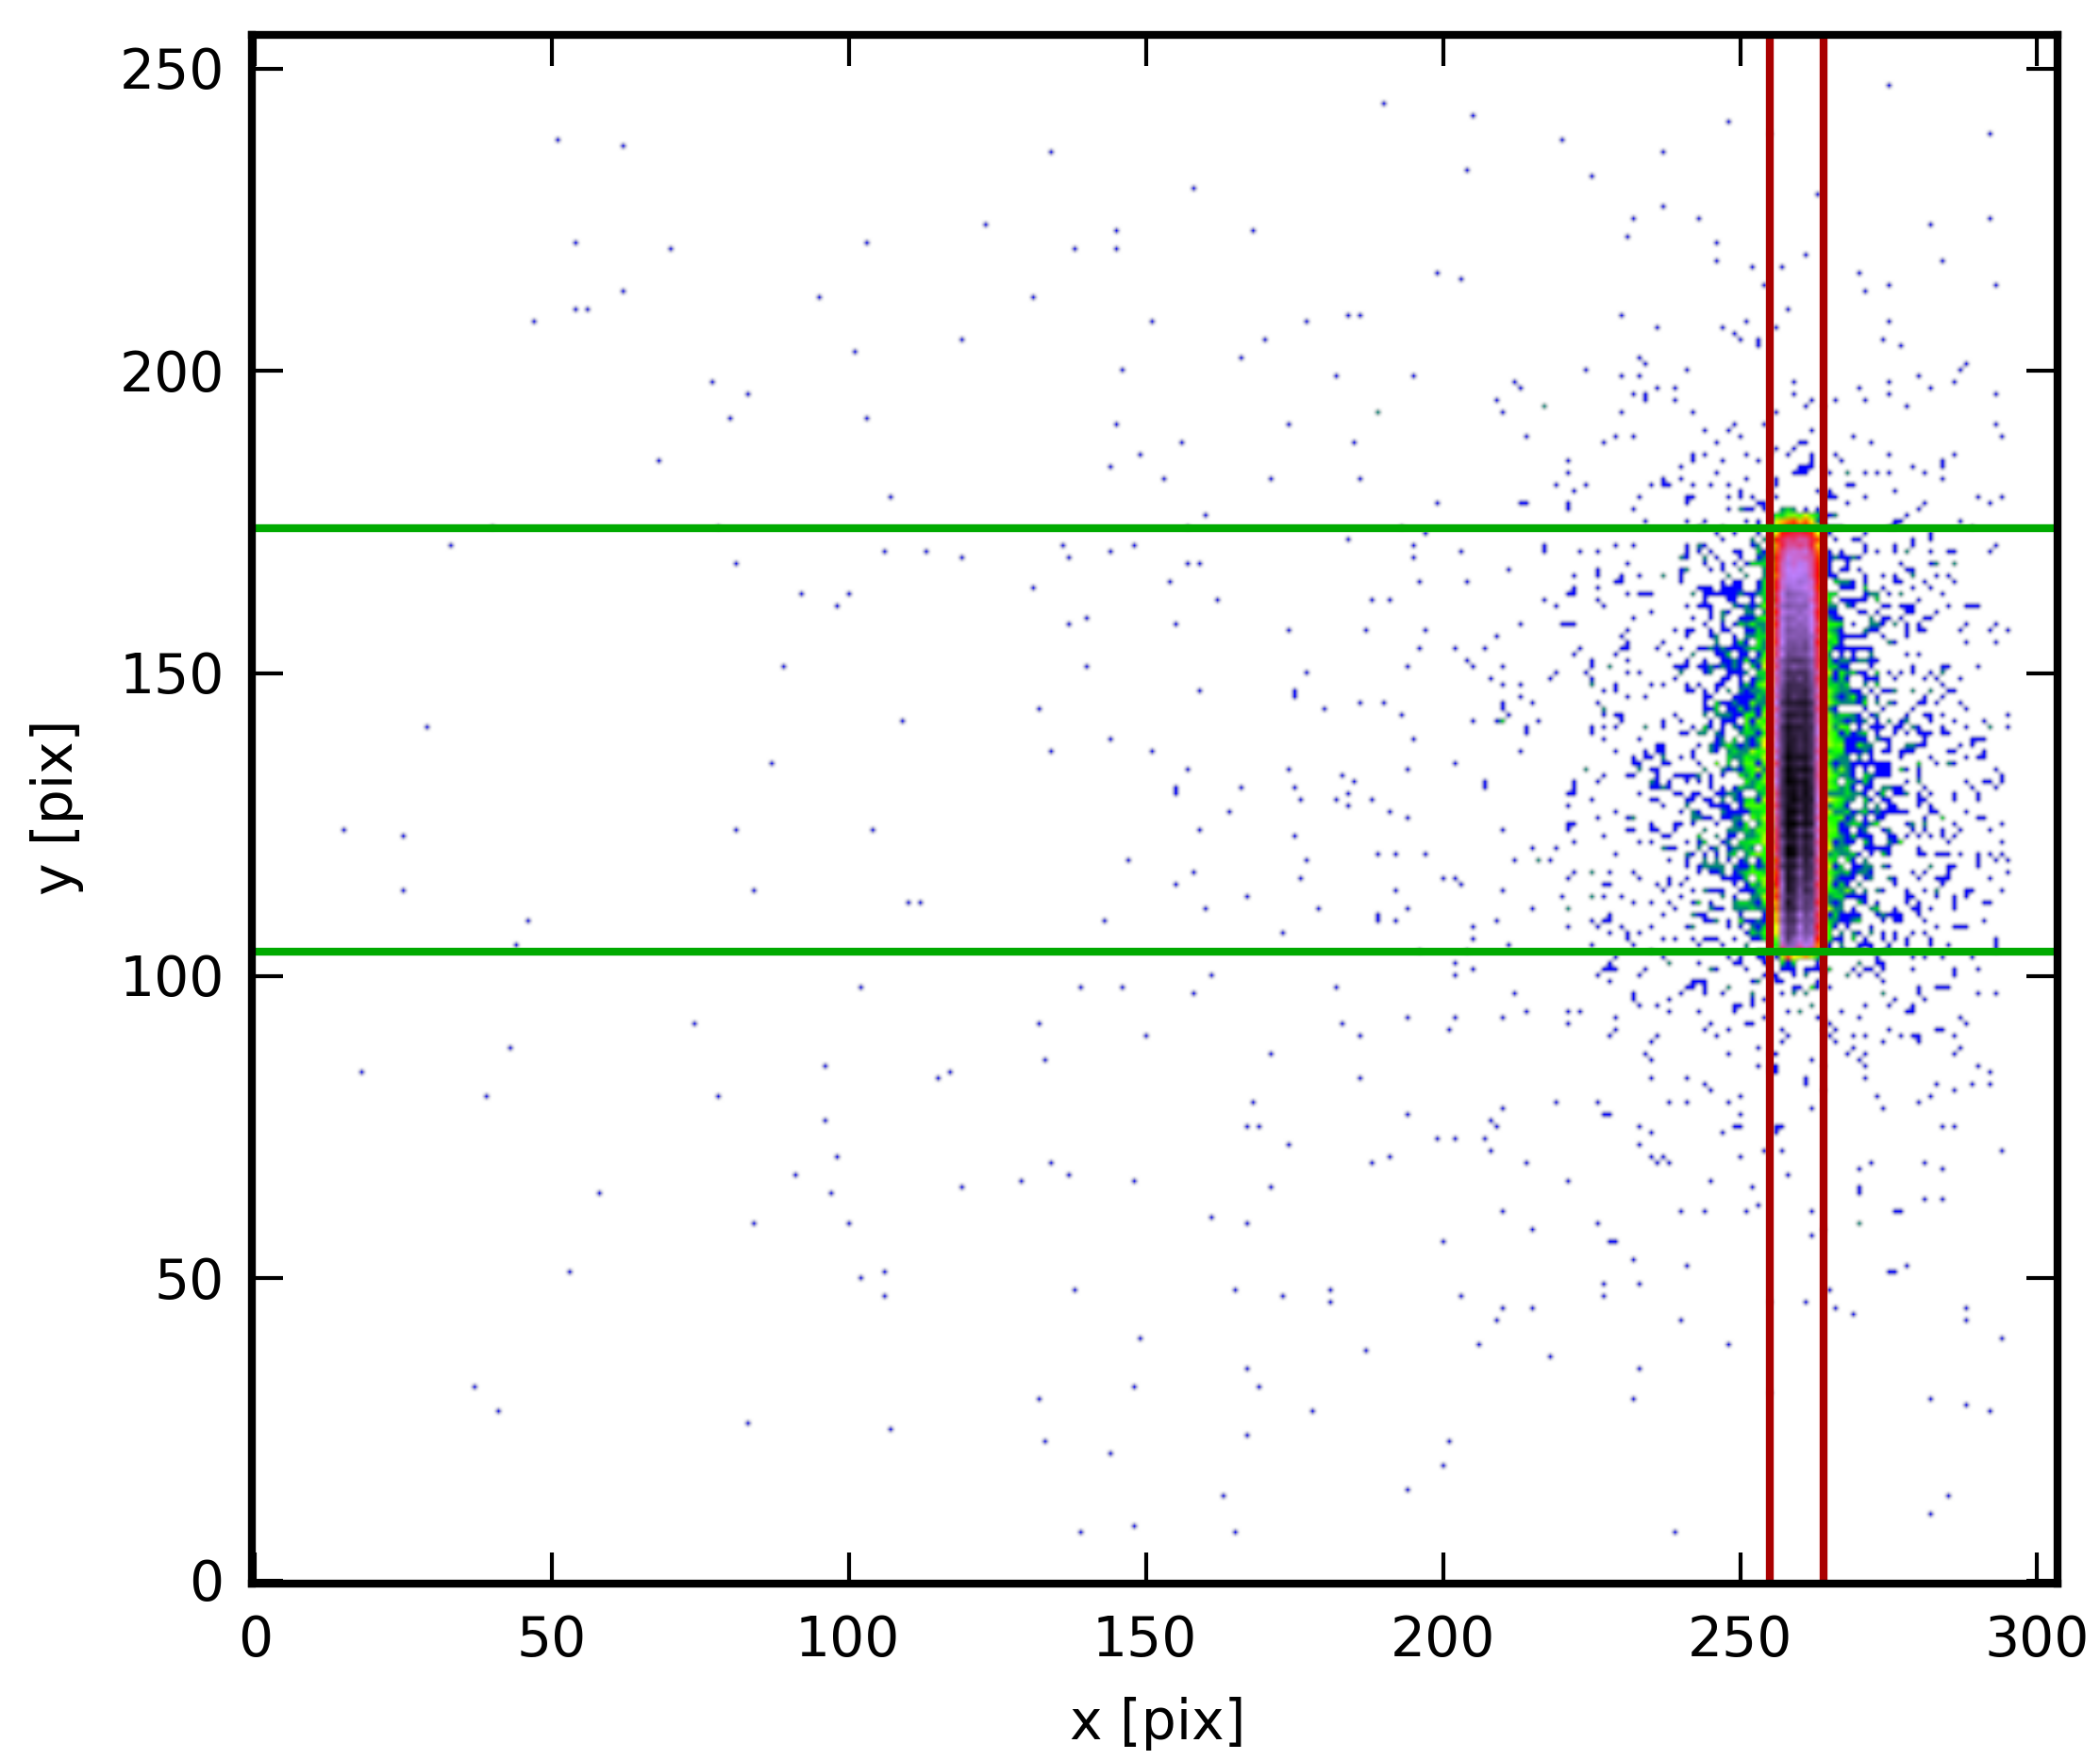
\includegraphics[width=155pt]{screenshots/normalizemap1.png} &
  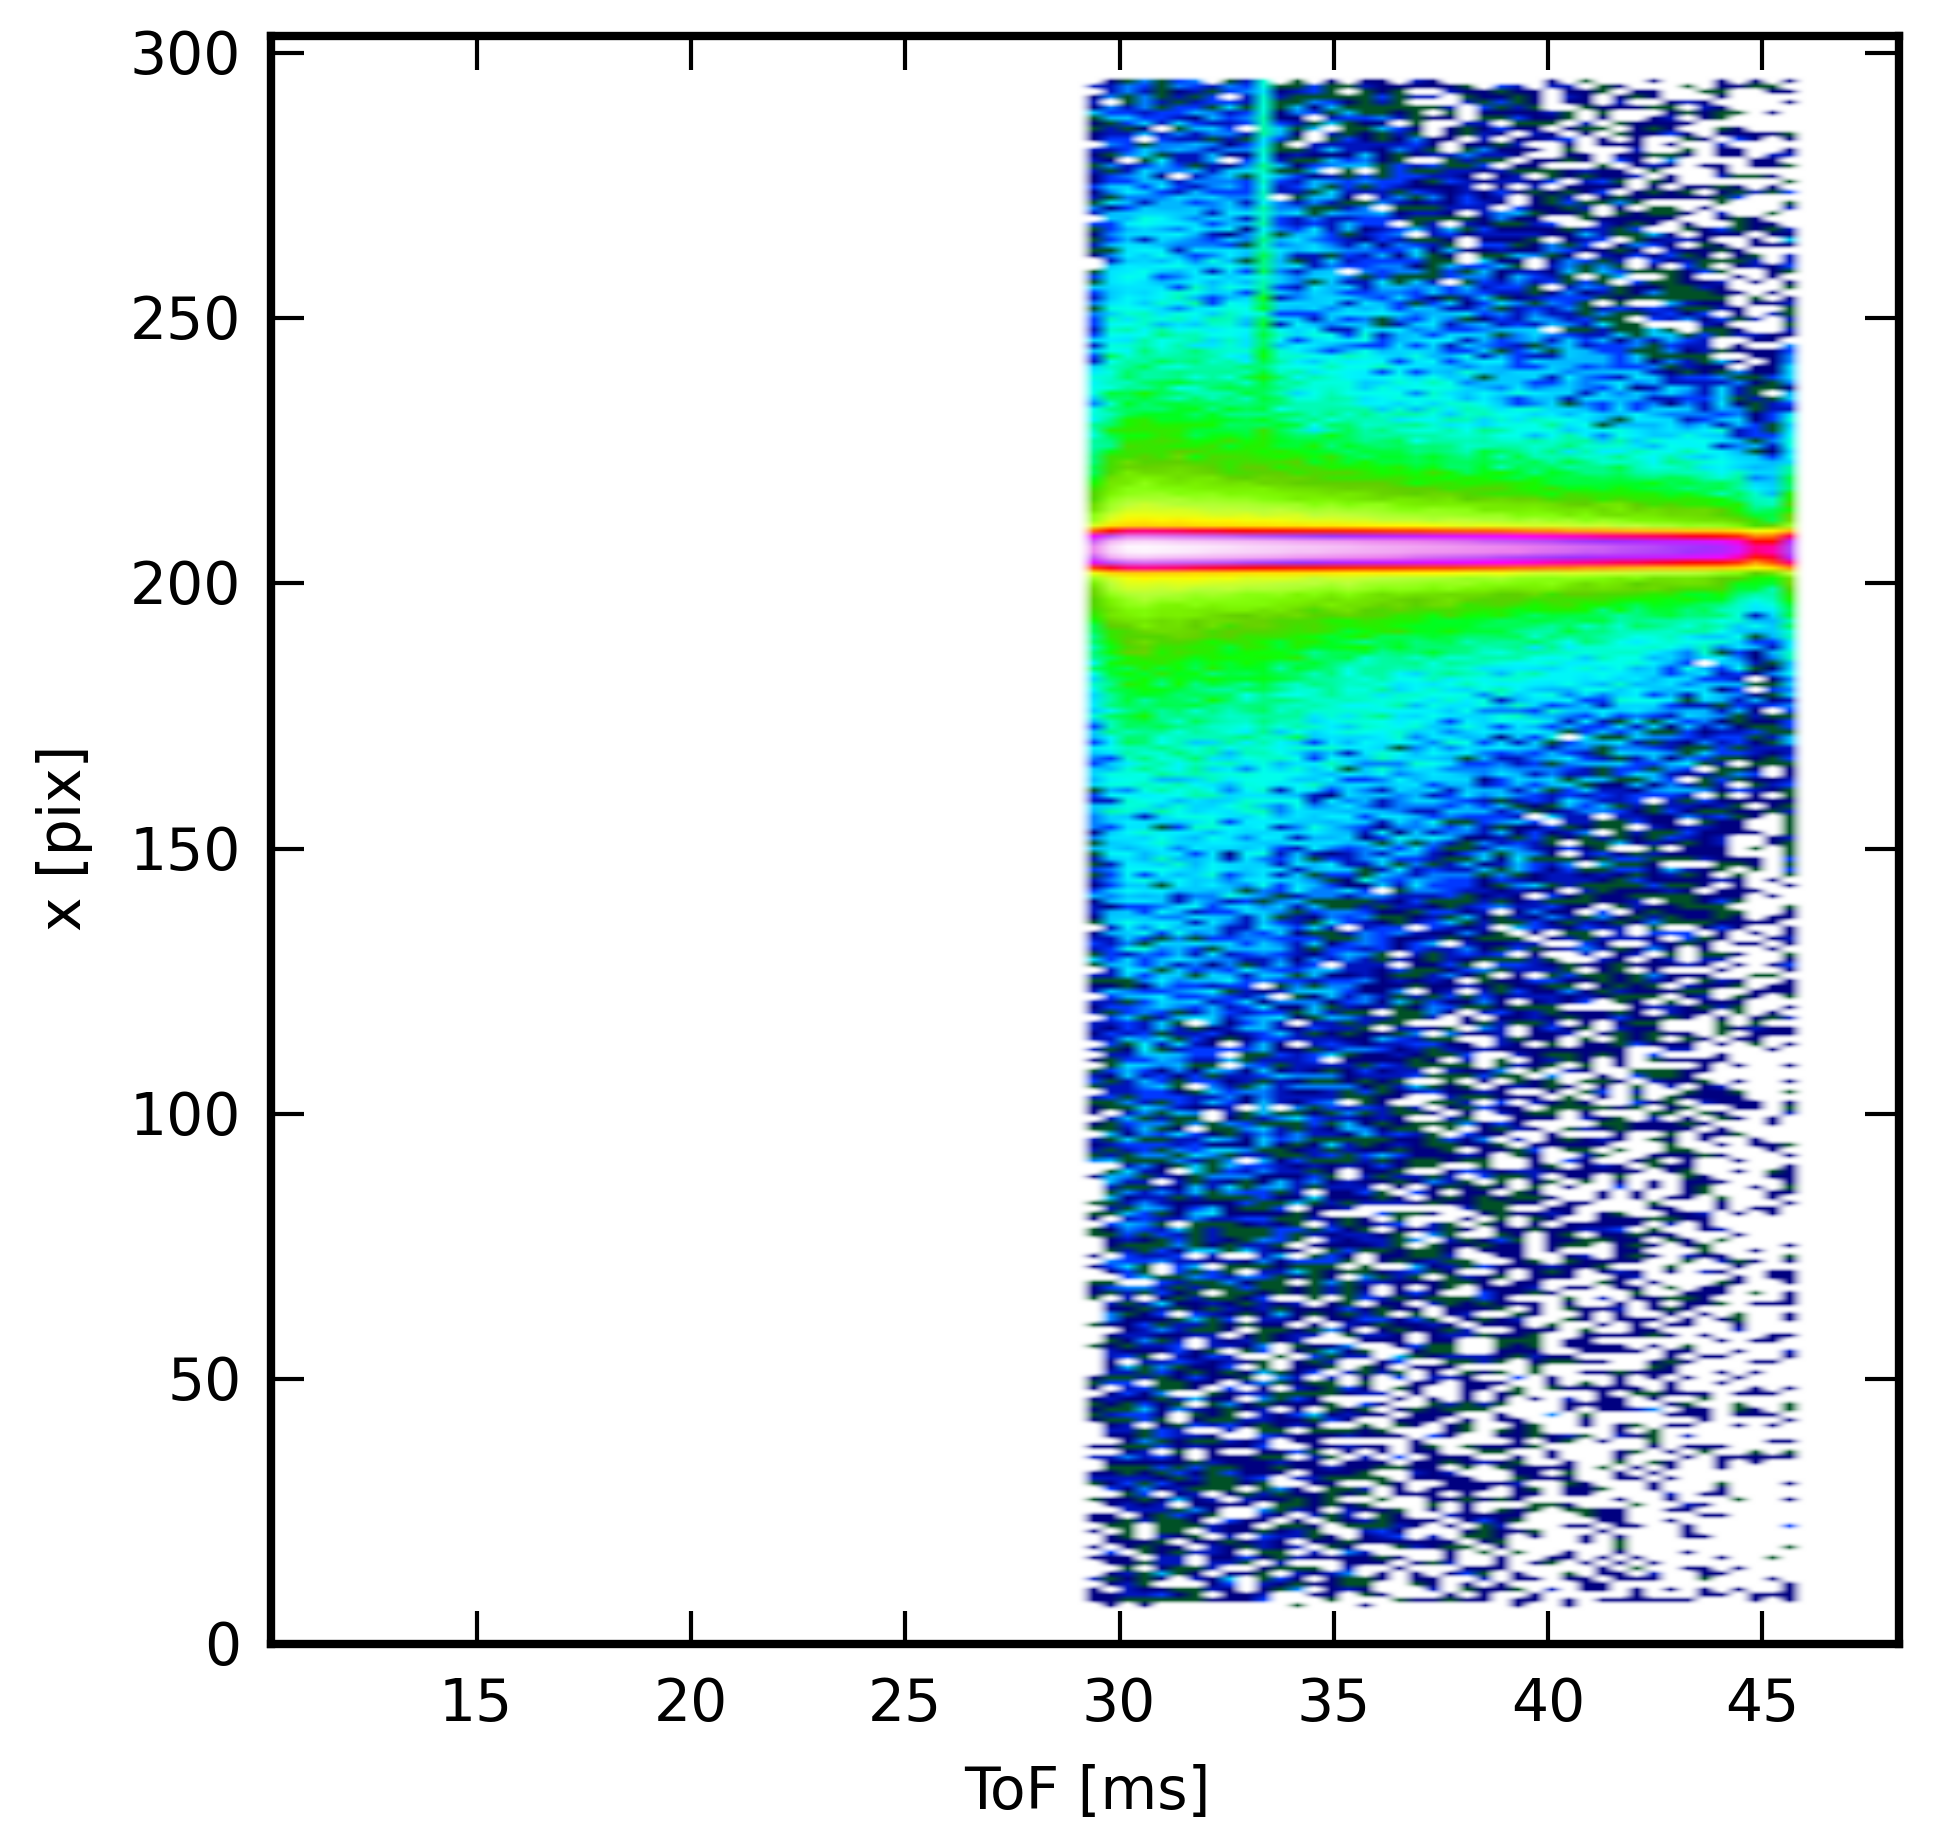
\includegraphics[width=155pt]{screenshots/normalizemap2.png} &\\
  Overview X-Y & Overview ToF-X & \\
  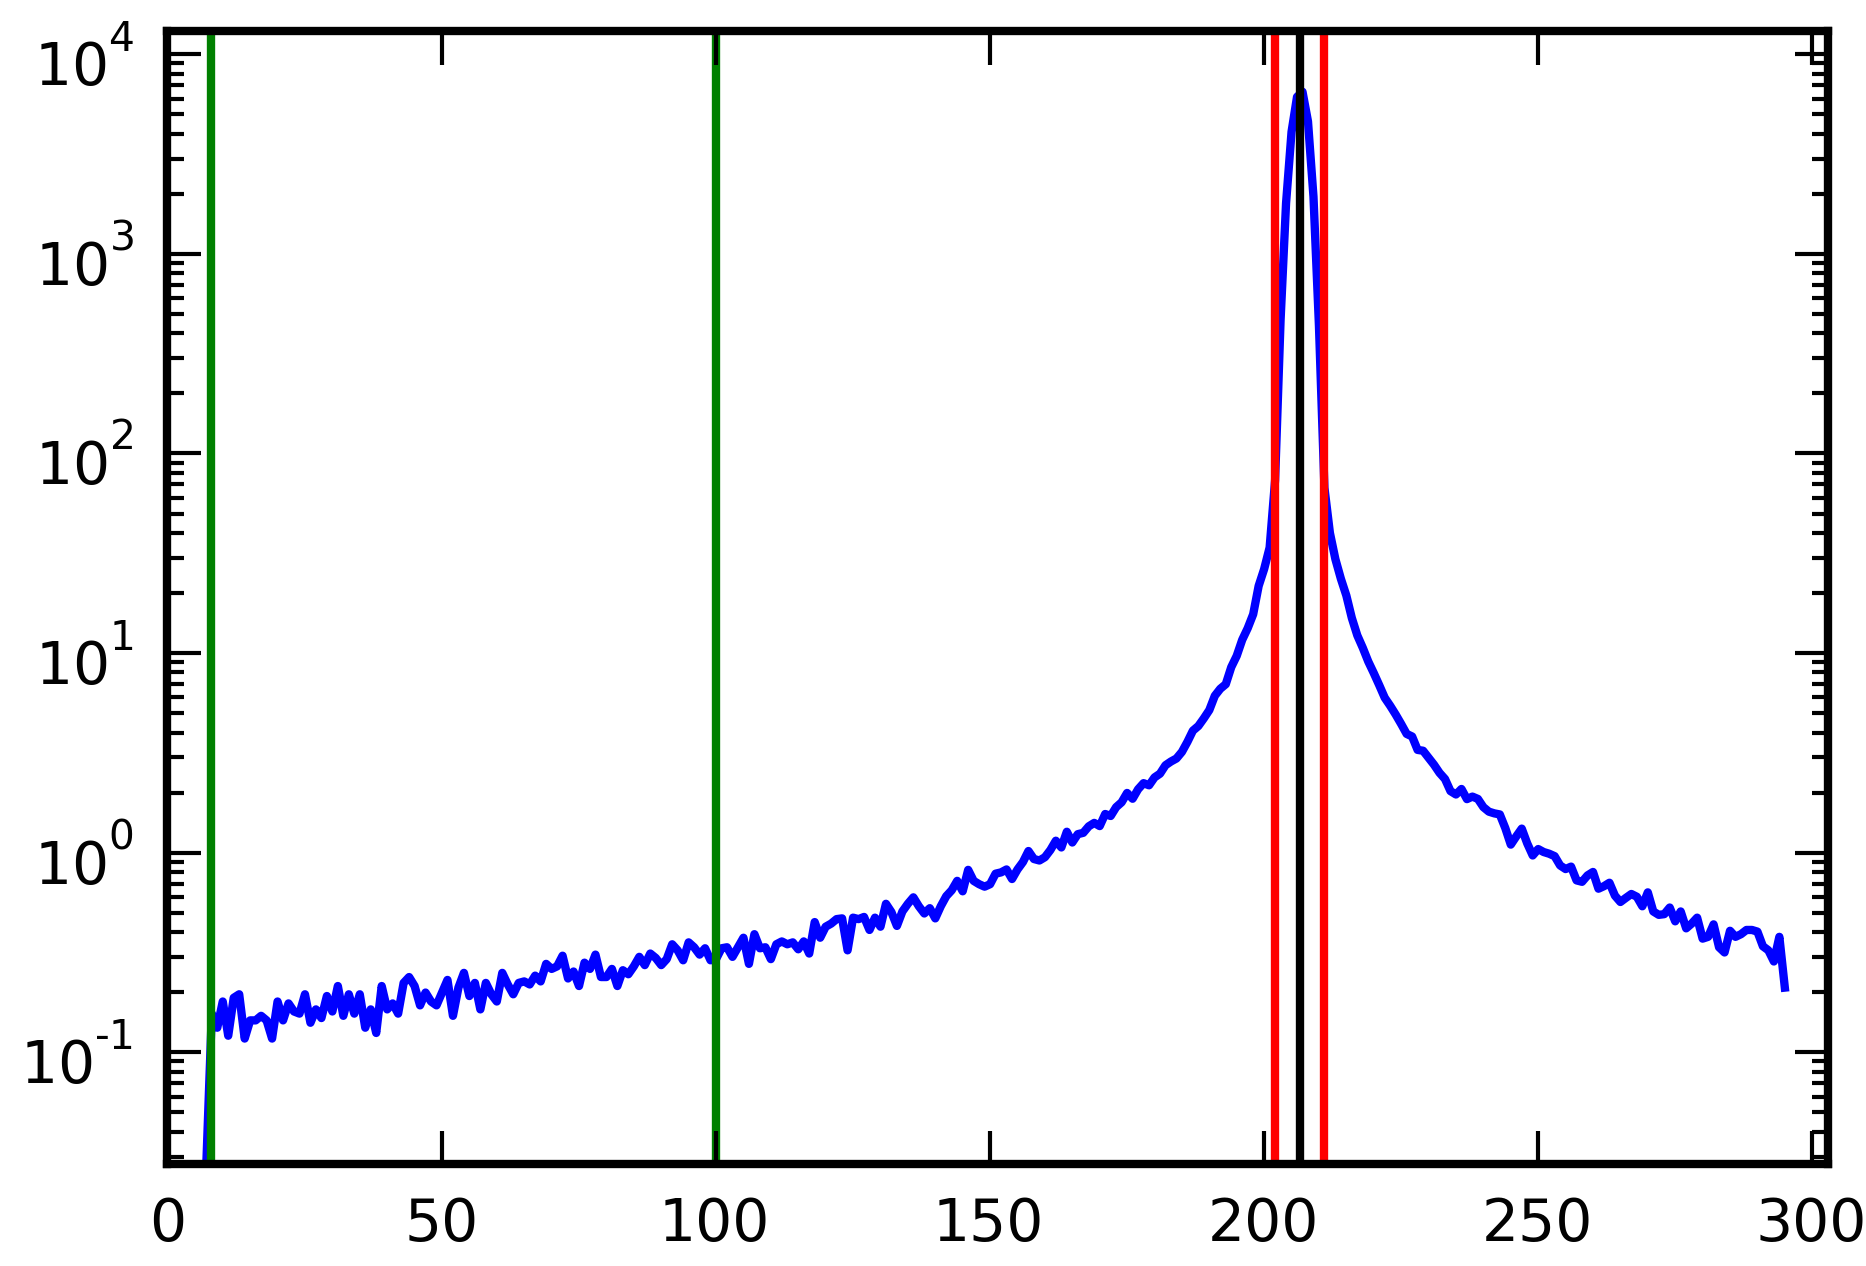
\includegraphics[width=155pt]{screenshots/normalize1.png} &
  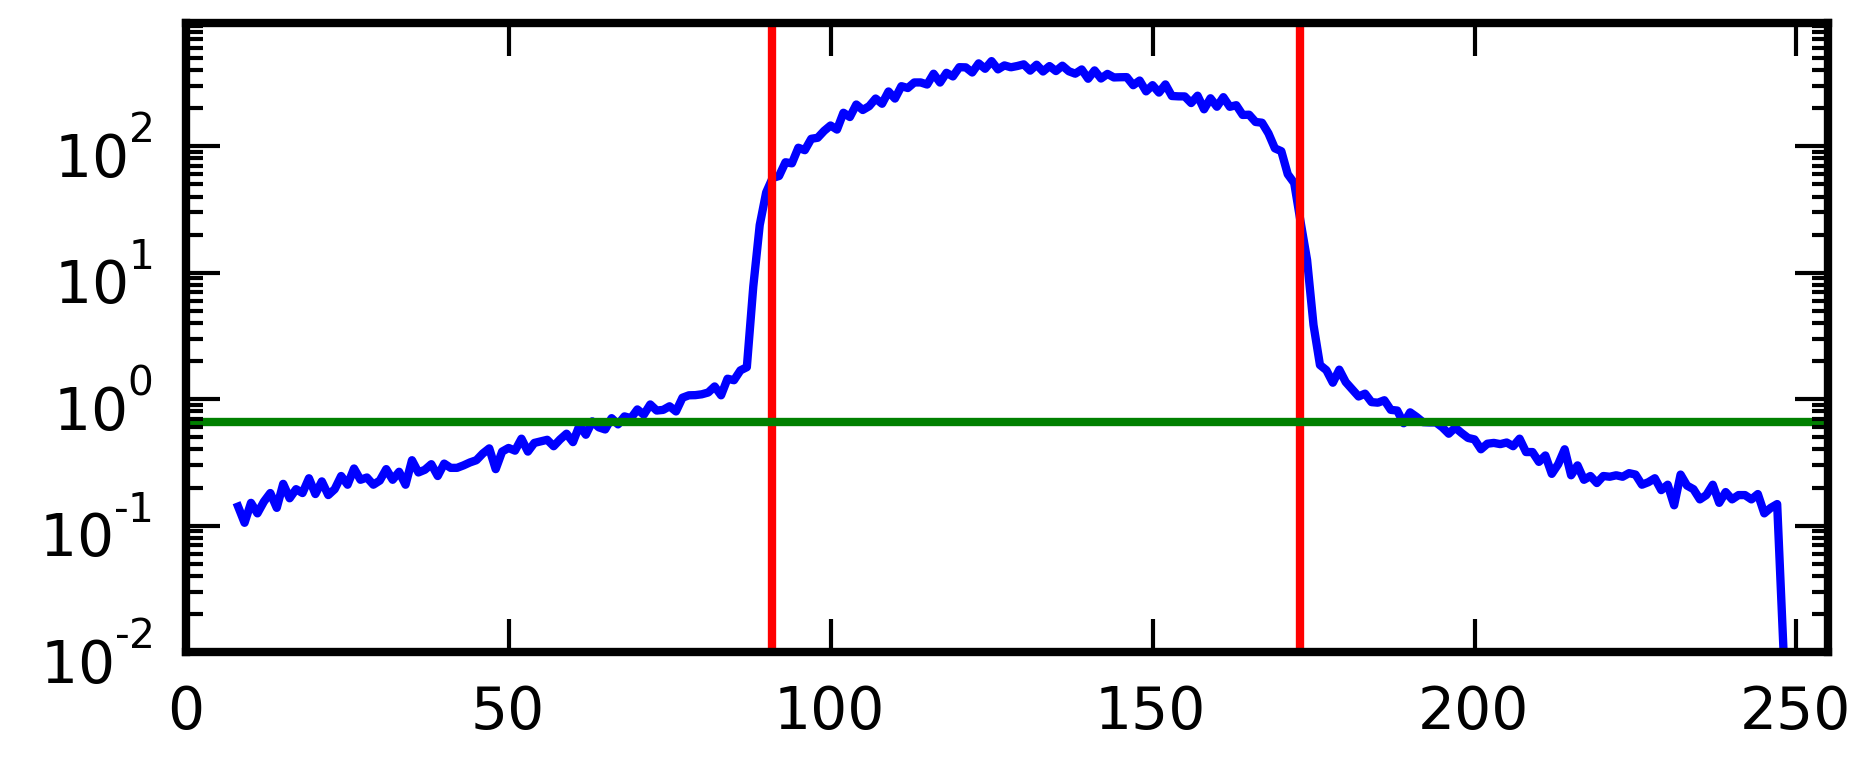
\includegraphics[width=155pt]{screenshots/normalize2.png} &
  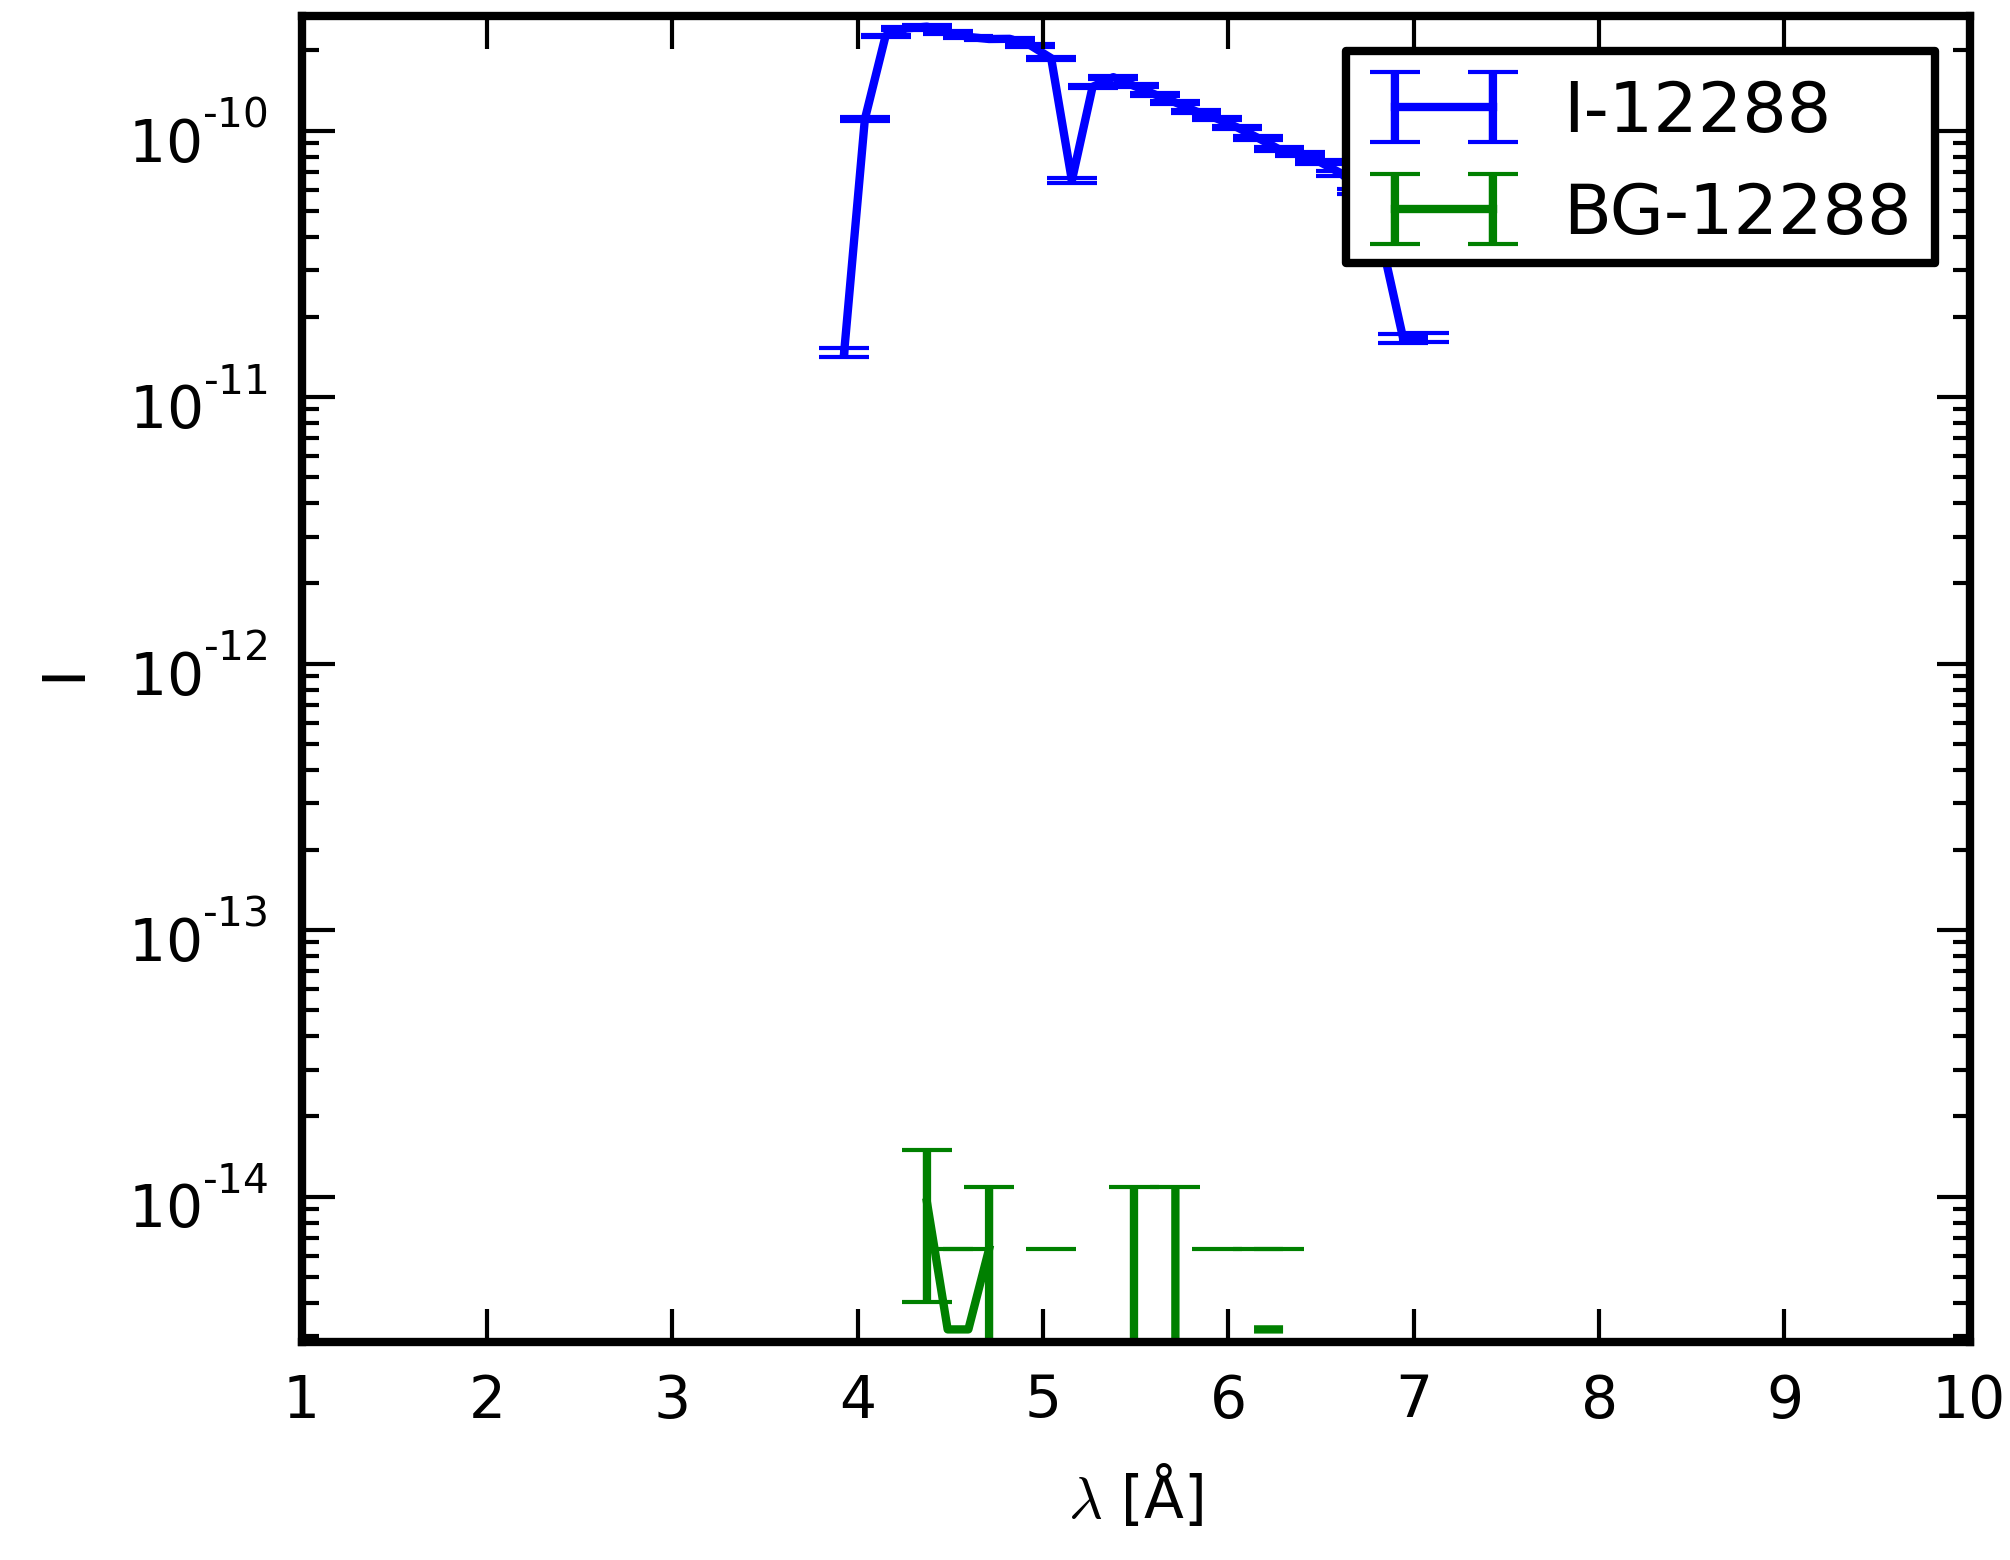
\includegraphics[width=120pt]{screenshots/normalize3.png} \\
  X-Projection & Y-Projection & Reflectivity
  \end{tabular}



\section{Go full-automatic: Reduction for dummies}
  For good quality data (enough intensity and narrow reflection) the program supports a fully automatized mode, where all reduction parameters are automatically calculated.
  This mode will be applied automatically when more than one dataset is selected at the File Open Dialog.
  The direct beam measurement have to have lower scan numbers than the actual measurements or need to be set in advance for this method to work.
  
  The automatic algorithm performs the same steps as described in section \ref{sec:quick_start}, while trying to guess the best parameters.
  The datasets are read one-by-one and, depending on the reflection angle, they are either set as normalization or reflectivity data in the reduction list.
  Here is an example how the interface might look after the algorithm has finished:
  
  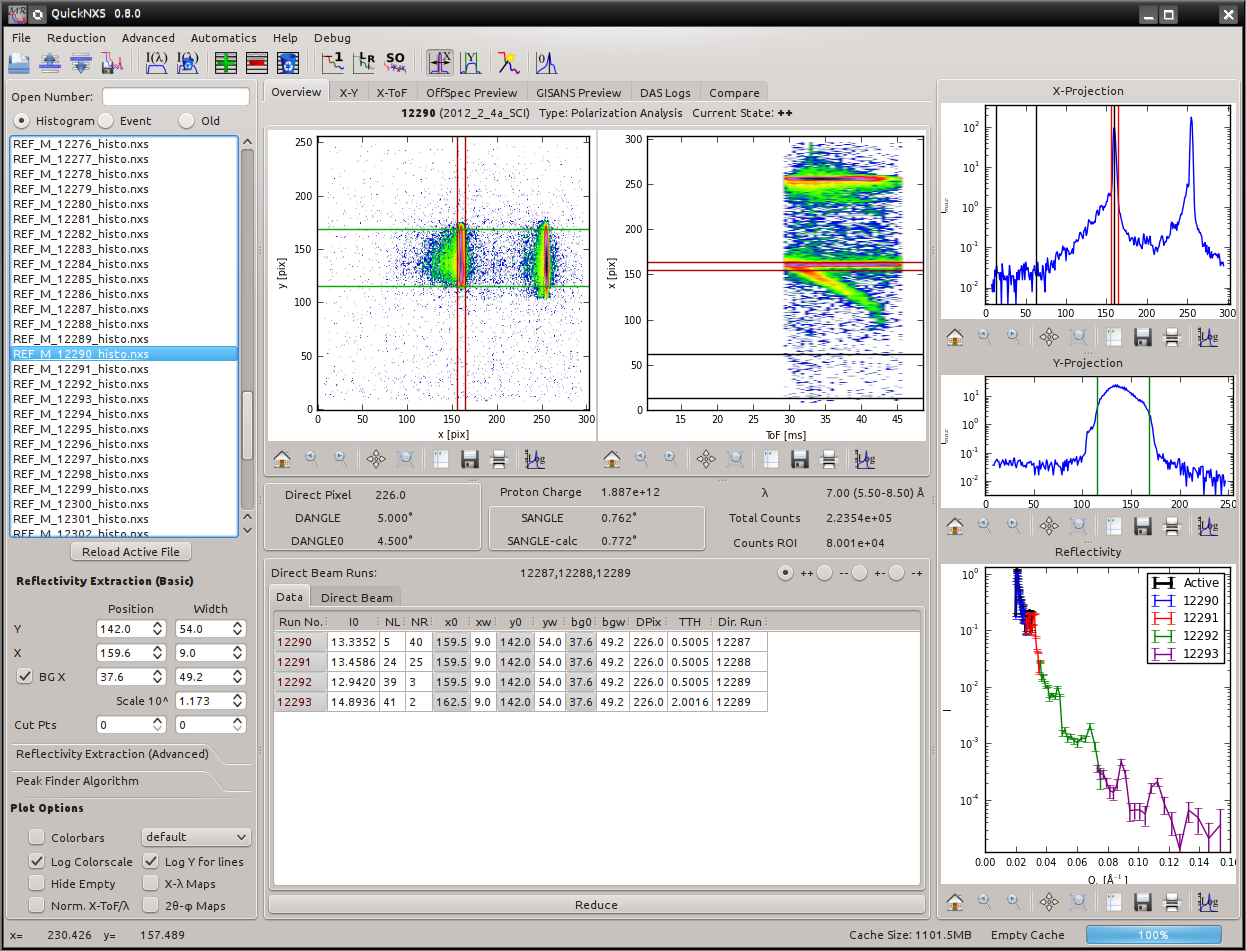
\includegraphics[width=460pt]{screenshots/overview.png}
  
  
  You can now scale individual datasets as described in \ref{sec:scaling}, if the stitching was not performed optimally.
  When satisfied with the result, you can save the data as described in the export section \ref{sec:export}.
  

\section{Quick start: Step-by-step standard reduction}
\label{sec:quick_start}
  For most datasets the reduction is done very similar to the fully automatized method but with more control of the user.
  Every dataset is examined by the operator to select the best extraction parameters.
  
  \subsection{Step 1: Set wavelength normalization from direct beam}
    \begin{wrapfigure}[11]{r}{0.55\textwidth}
    \begin{tabular}{cc}
        Reflectivity before & Reflectivity after \\
      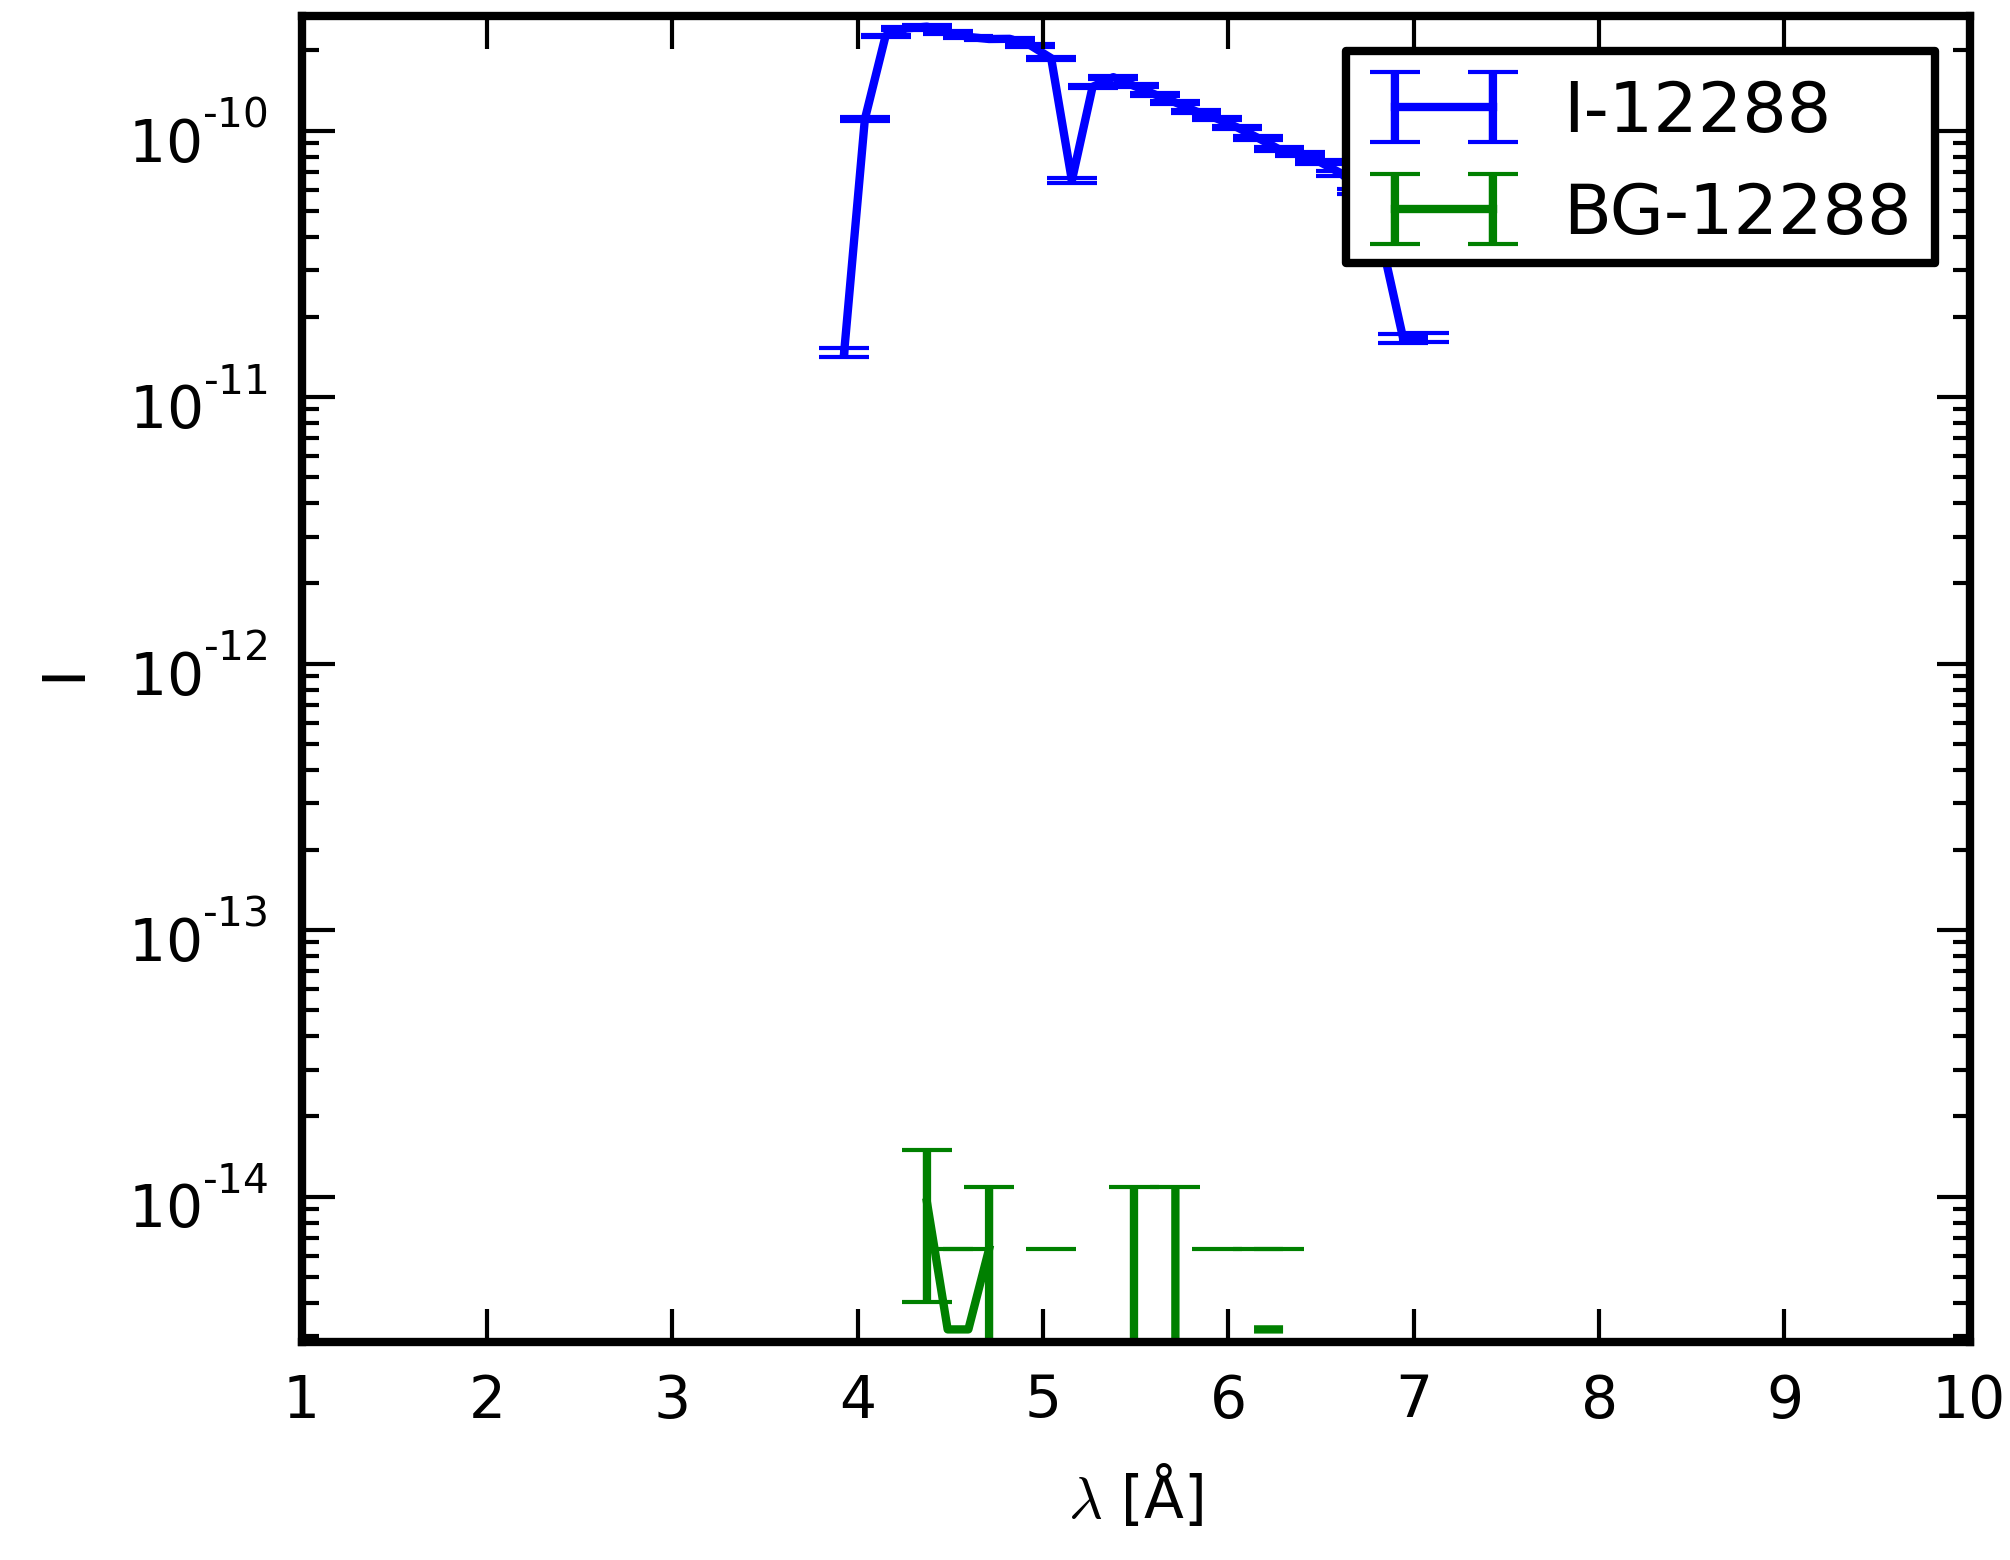
\includegraphics[width=115pt]{screenshots/normalize3.png} & 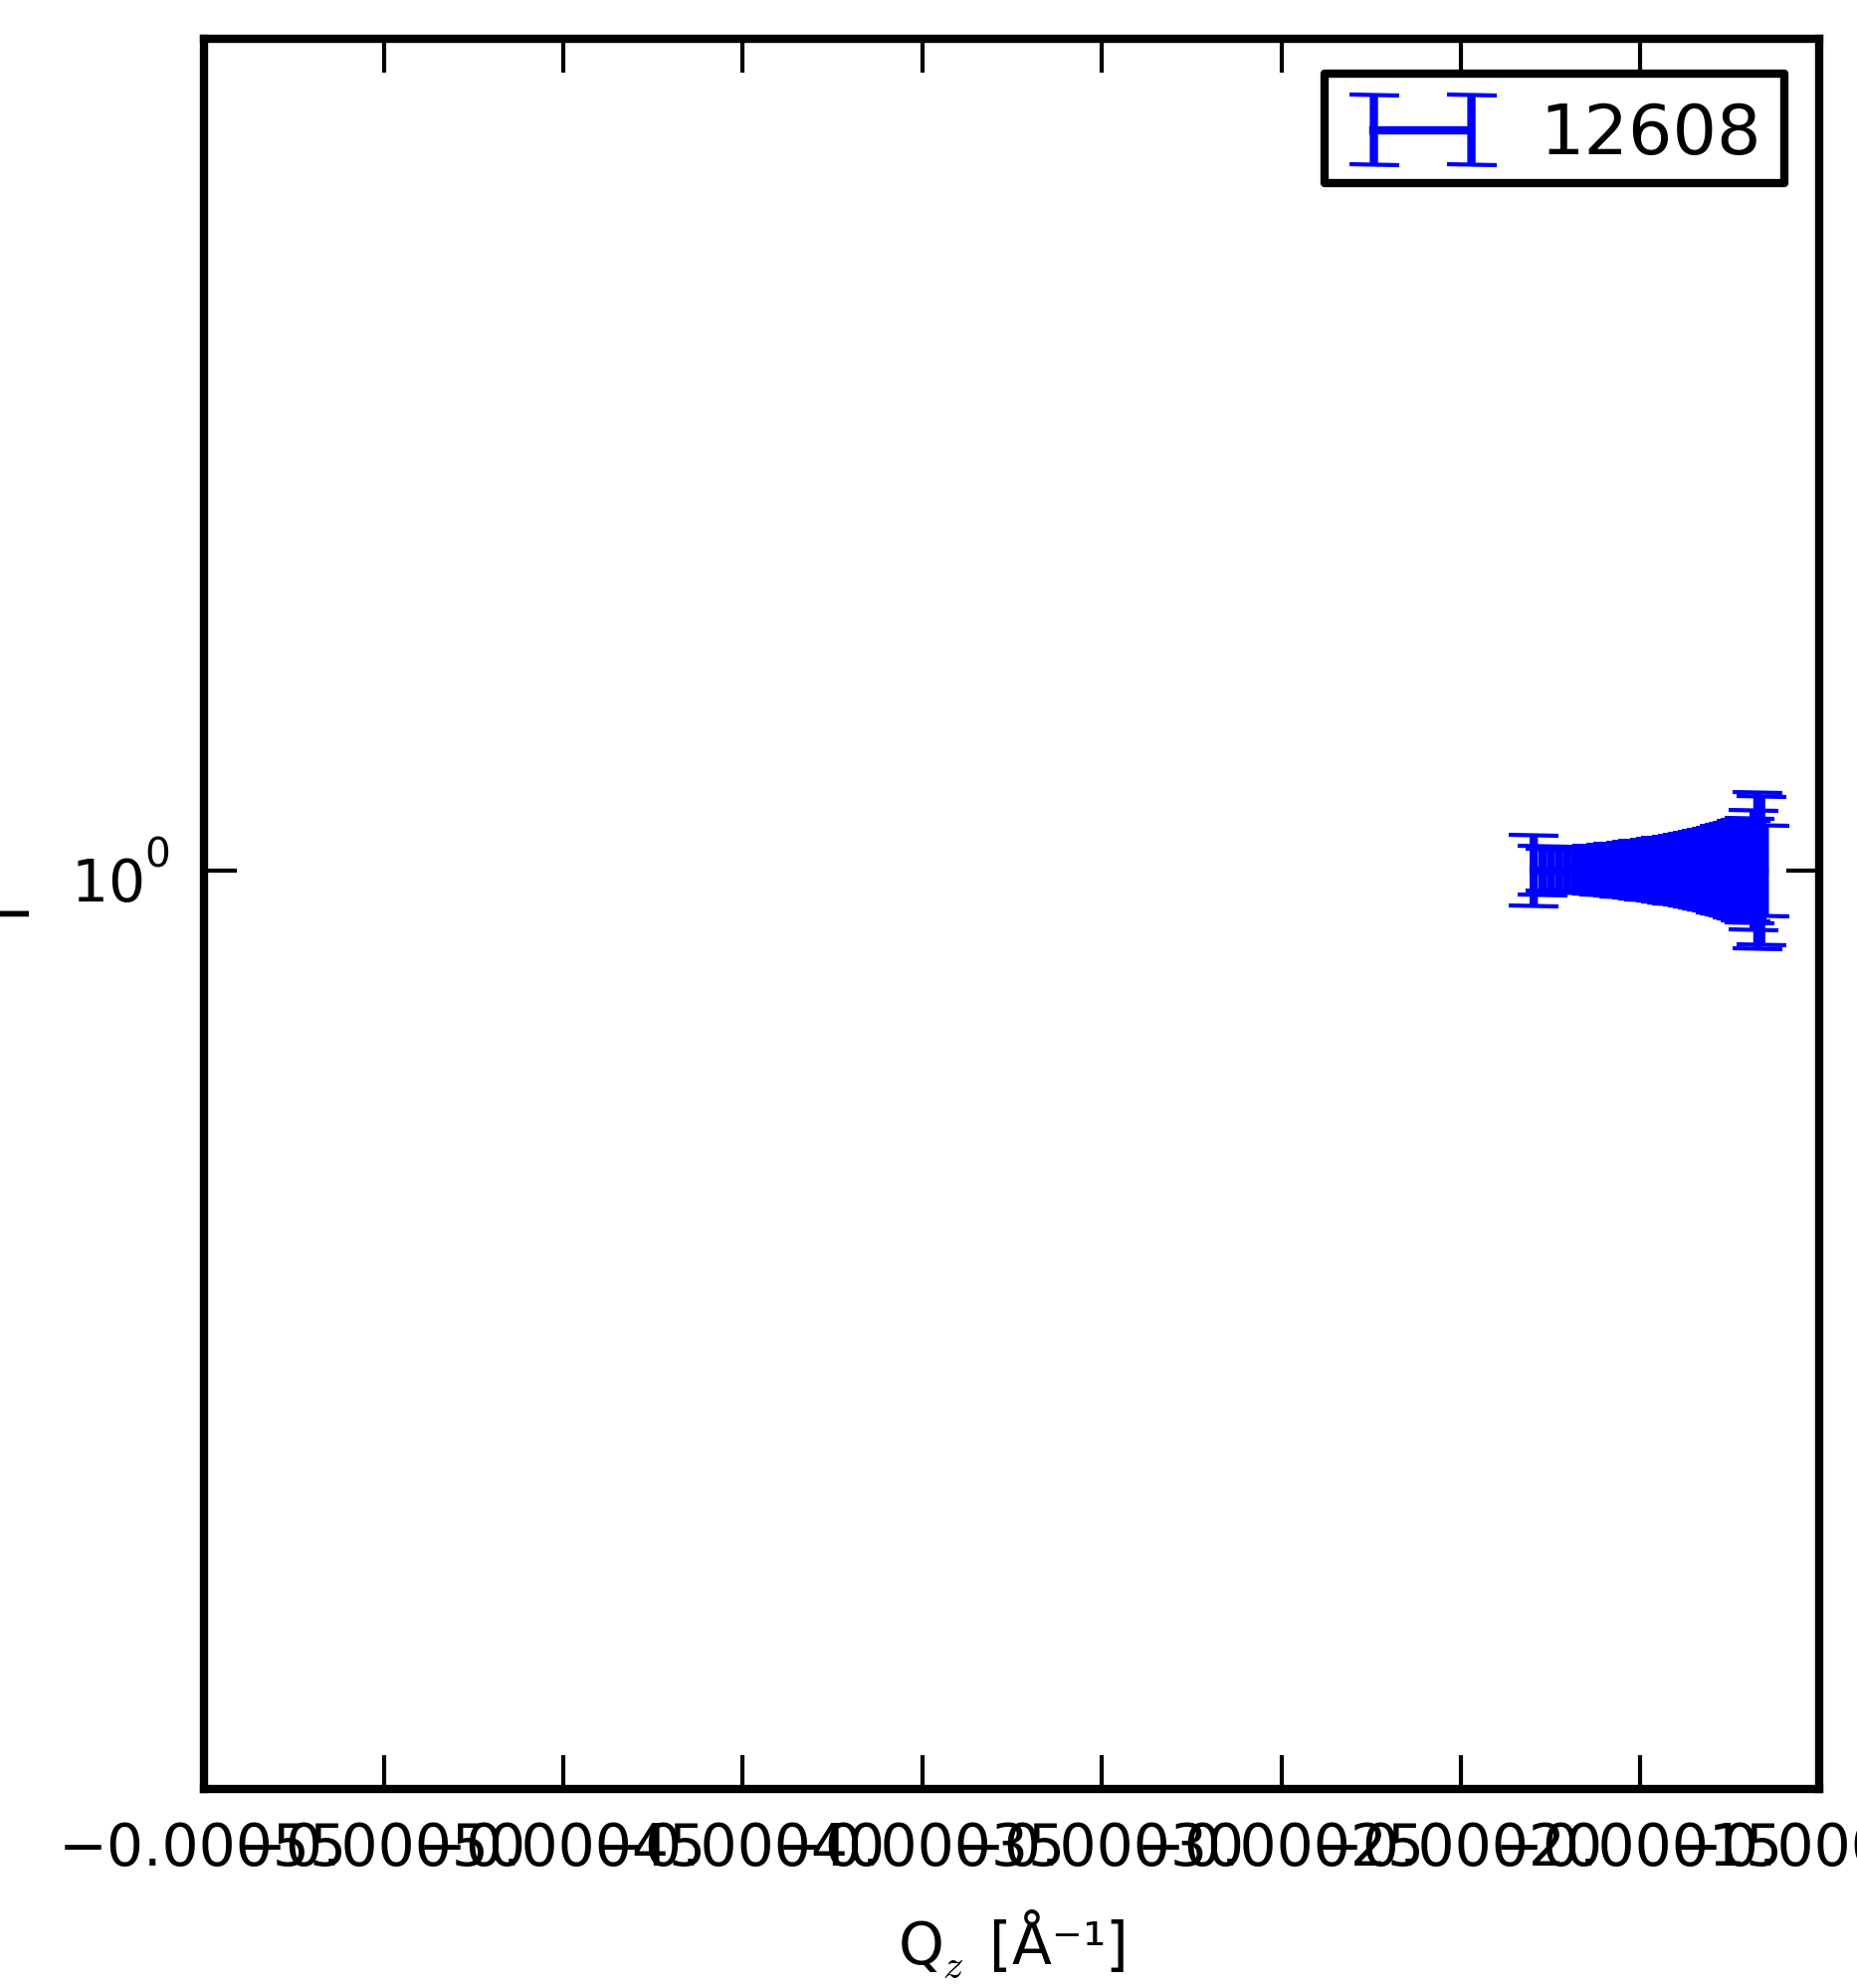
\includegraphics[width=115pt]{screenshots/normalize_after.png}
    \end{tabular}     
    \end{wrapfigure}
  
        \textbf{Open your normalization file} as described in section \ref{sec:open_file}. 
      Make sure the SANGLE-calc value shown in the overview tab is close to zero and that the X- and Y-projections show the correct regions with the red indicators.
      Activate the \textbf{Set Normalization action} \icon{extractNormalization}, this will add the current dataset to the "Normalization" list, the "Direct Beam Runs:" label will show the number of the dataset and the reflectivity will show the normalized intensities, which should all be one.
      Repeat this step for each direct beam measurement needed for your dataset.

  
  \subsection{Step 2: Define a suitable background- and y-region}
    \begin{wrapfigure}[15]{r}{0.55\textwidth}
    \centering
      X-projection with background region (green)\\
      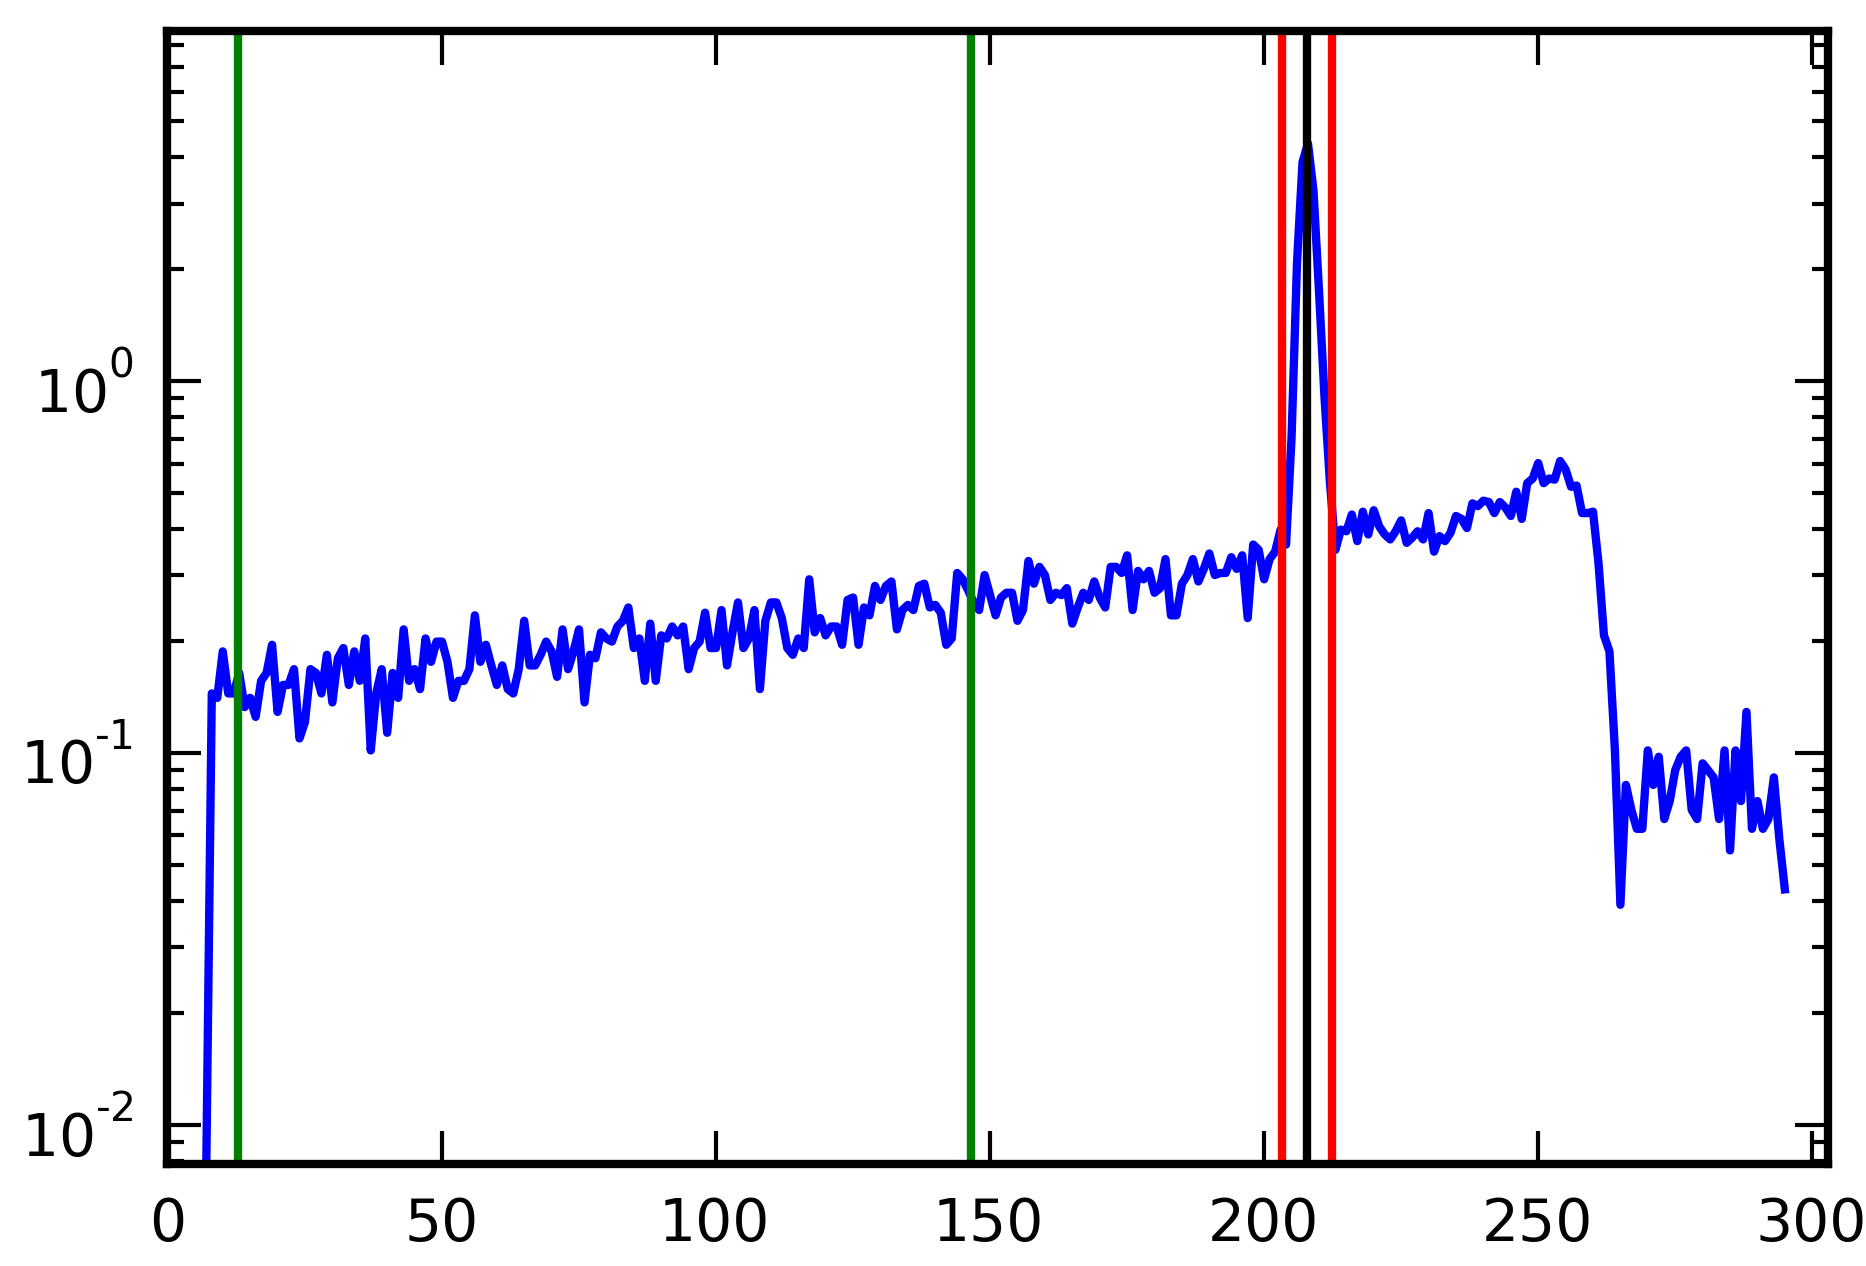
\includegraphics[width=160pt]{screenshots/background.png}
    \begin{tabular}{cc}
        Y-projection of small sample & X-Y map \\
      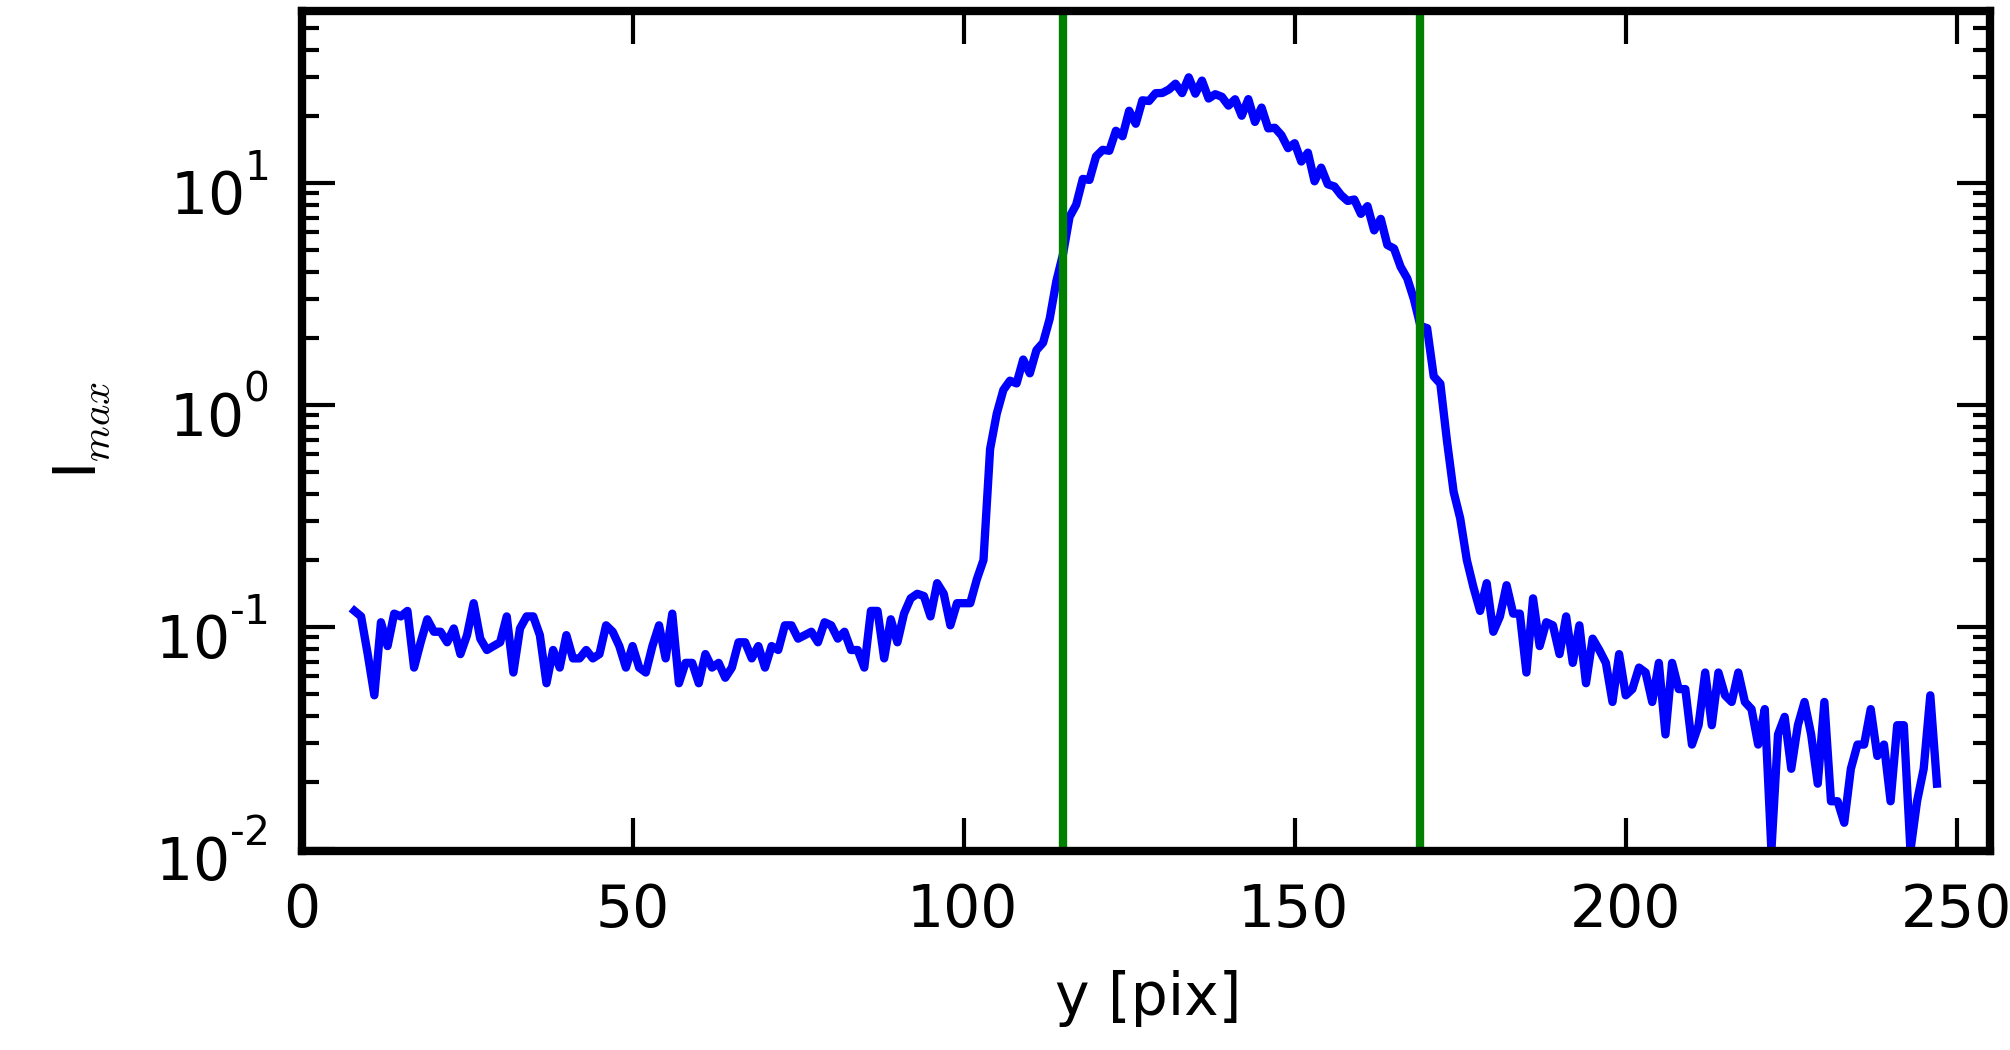
\includegraphics[width=160pt]{screenshots/yregion.png} & 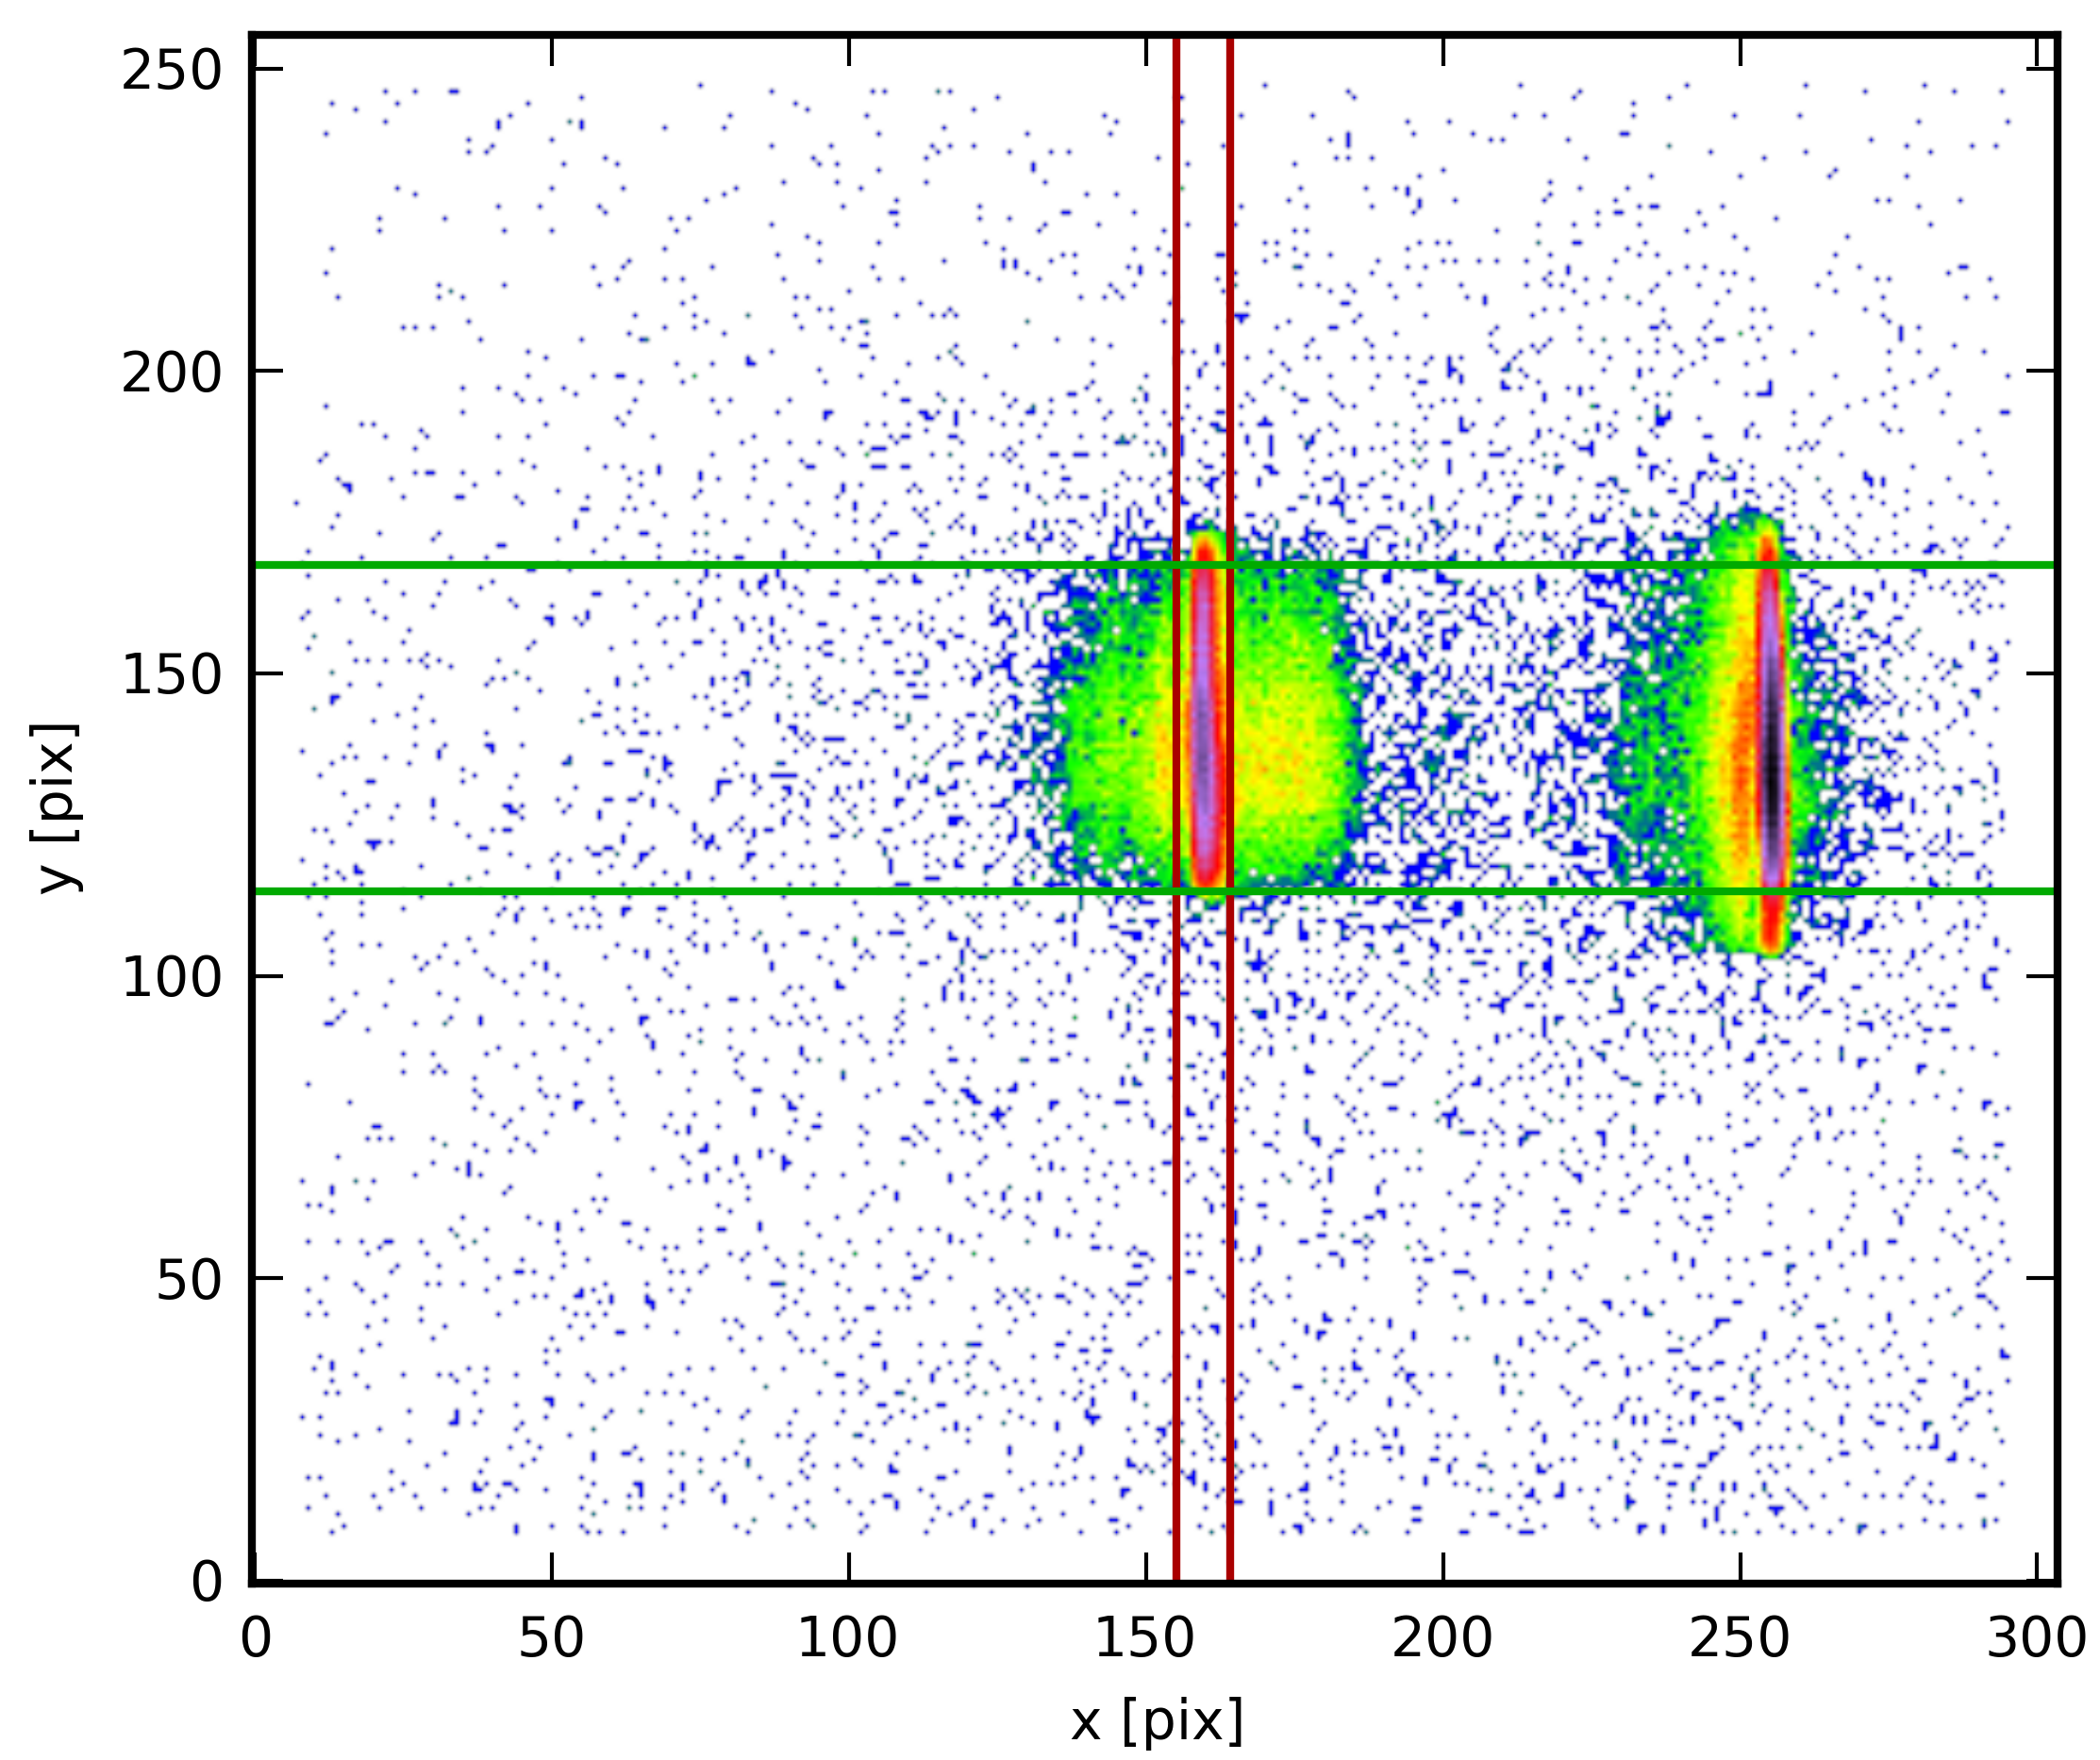
\includegraphics[width=70pt]{screenshots/yregionmap.png}
    \end{tabular}     
    \end{wrapfigure}
  
    Although it is in principle possible to define the extraction and background region for each dataset separately, it is recommended to use the same parameters for all files.
    From this perspective it is often a good idea to start with the dataset with the highest incident angle, as there the signal to background ration is the lowest.
    To produce the best results you should select a large region (statistics), keeping enough distance from the reflected beam (especially when off-specular Bragg-sheets are present) and to not include regions where the background drops (shadowed by the right detector slit for example).
    The Y-region, shown in the Y-projection of the first (low Q) dataset, is often detected very well automatically.
    Just check that it fits to the reflected intensity area. 
    For very small samples it can sometimes make sense to manually restrain the area to the sample reflection.
  
  \subsection{Step 3: Normalize to total reflection and add the first dataset}
    \begin{wrapfigure}[13]{r}{0.4\textwidth}
     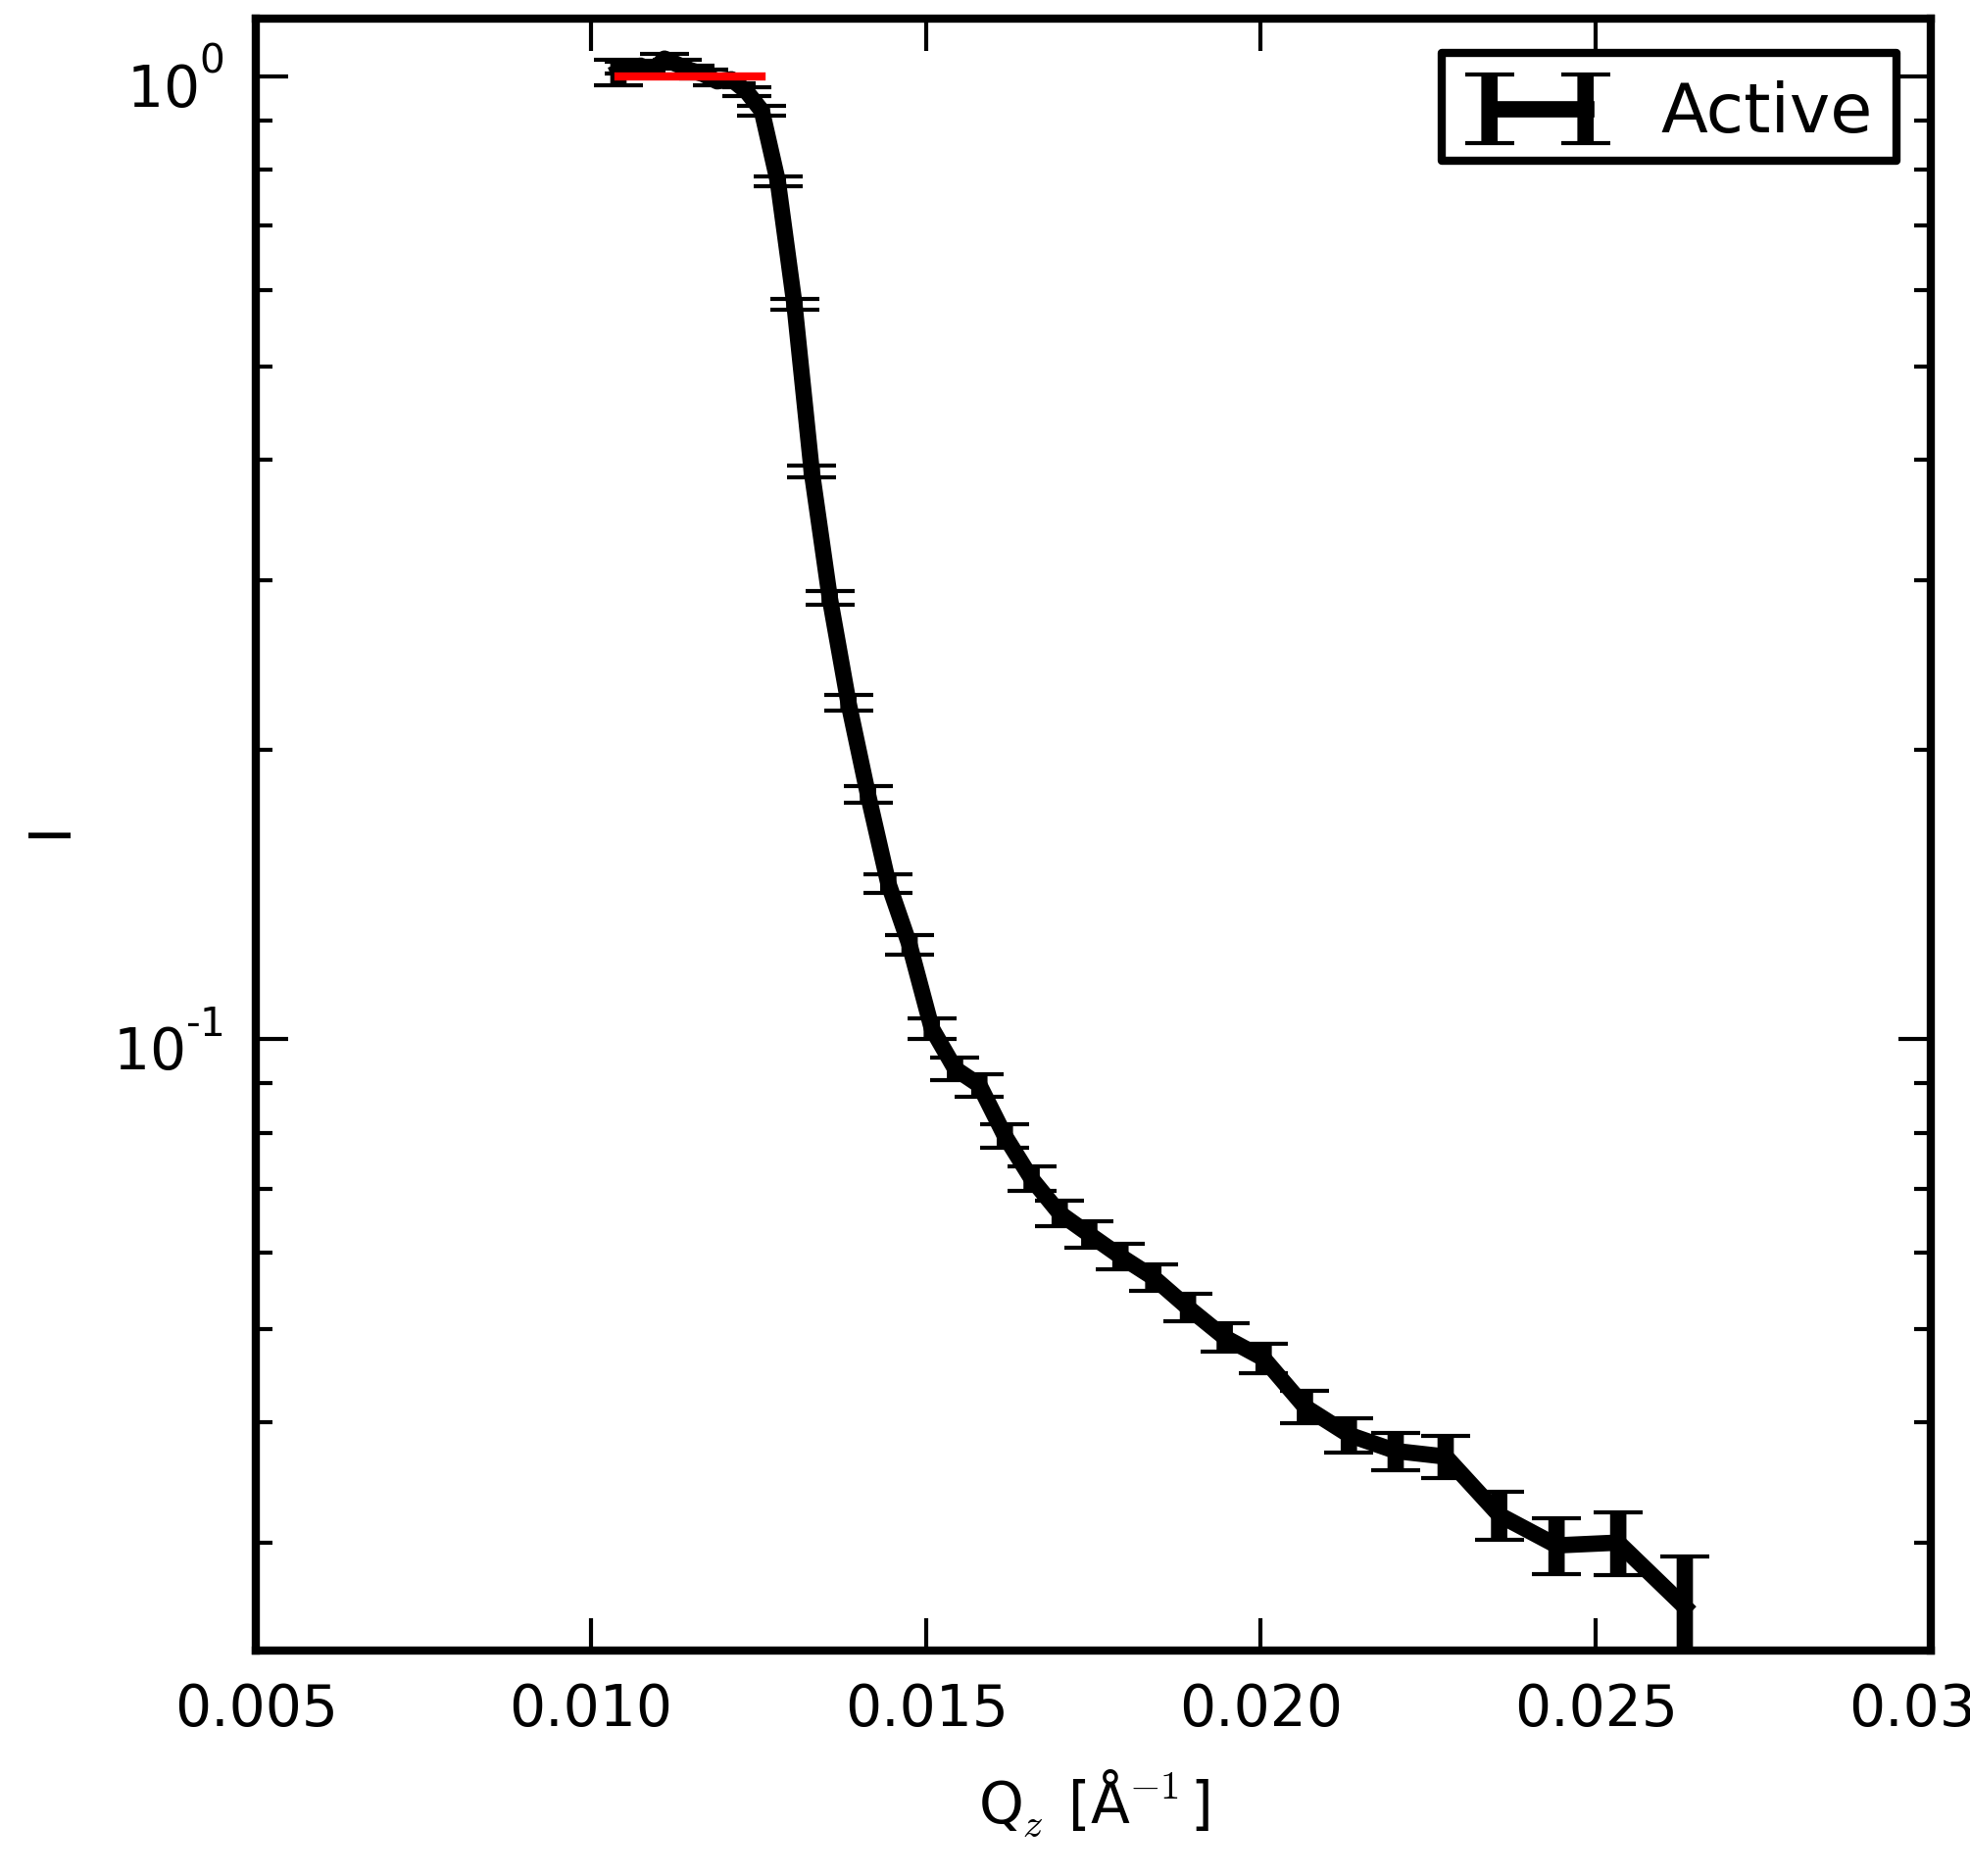
\includegraphics[width=165pt]{screenshots/totalreflection.png} 
    \end{wrapfigure}
    Go to your dataset starting at the lowest \Qz value, remove points from the low \Qz region, which are not reasonable with the \textbf{Cut Pts parameters}:
    
\includegraphics[width=115pt]{screenshots/cutpoints.png} (can be done automatically with the \textbf{Cut Points (L/R)} \icon{cutPoints} action). Than activate the \textbf{Set Scaling action} \icon{totalReflection} to normalize the total reflection to one.
    This should now look like the image on the right.
    Next add the dataset to the refinement list using the \textbf{Keep Item in List action} \icon{addRef} to add the dataset with the current parameters in the list.
    This will automatically switch off the \textbf{Automatic Y Limits} \icon{limitYauto}, so all datasets will be reduced with the same Y-range.
    This is important for the high \Qz region as the background often inhibits a good automatic detection of the Y-region.
    
  
  \subsection{Step 4: Add additional datasets and stitch them together}
    \begin{wrapfigure}[12]{r}{0.4\textwidth}
    \centering
     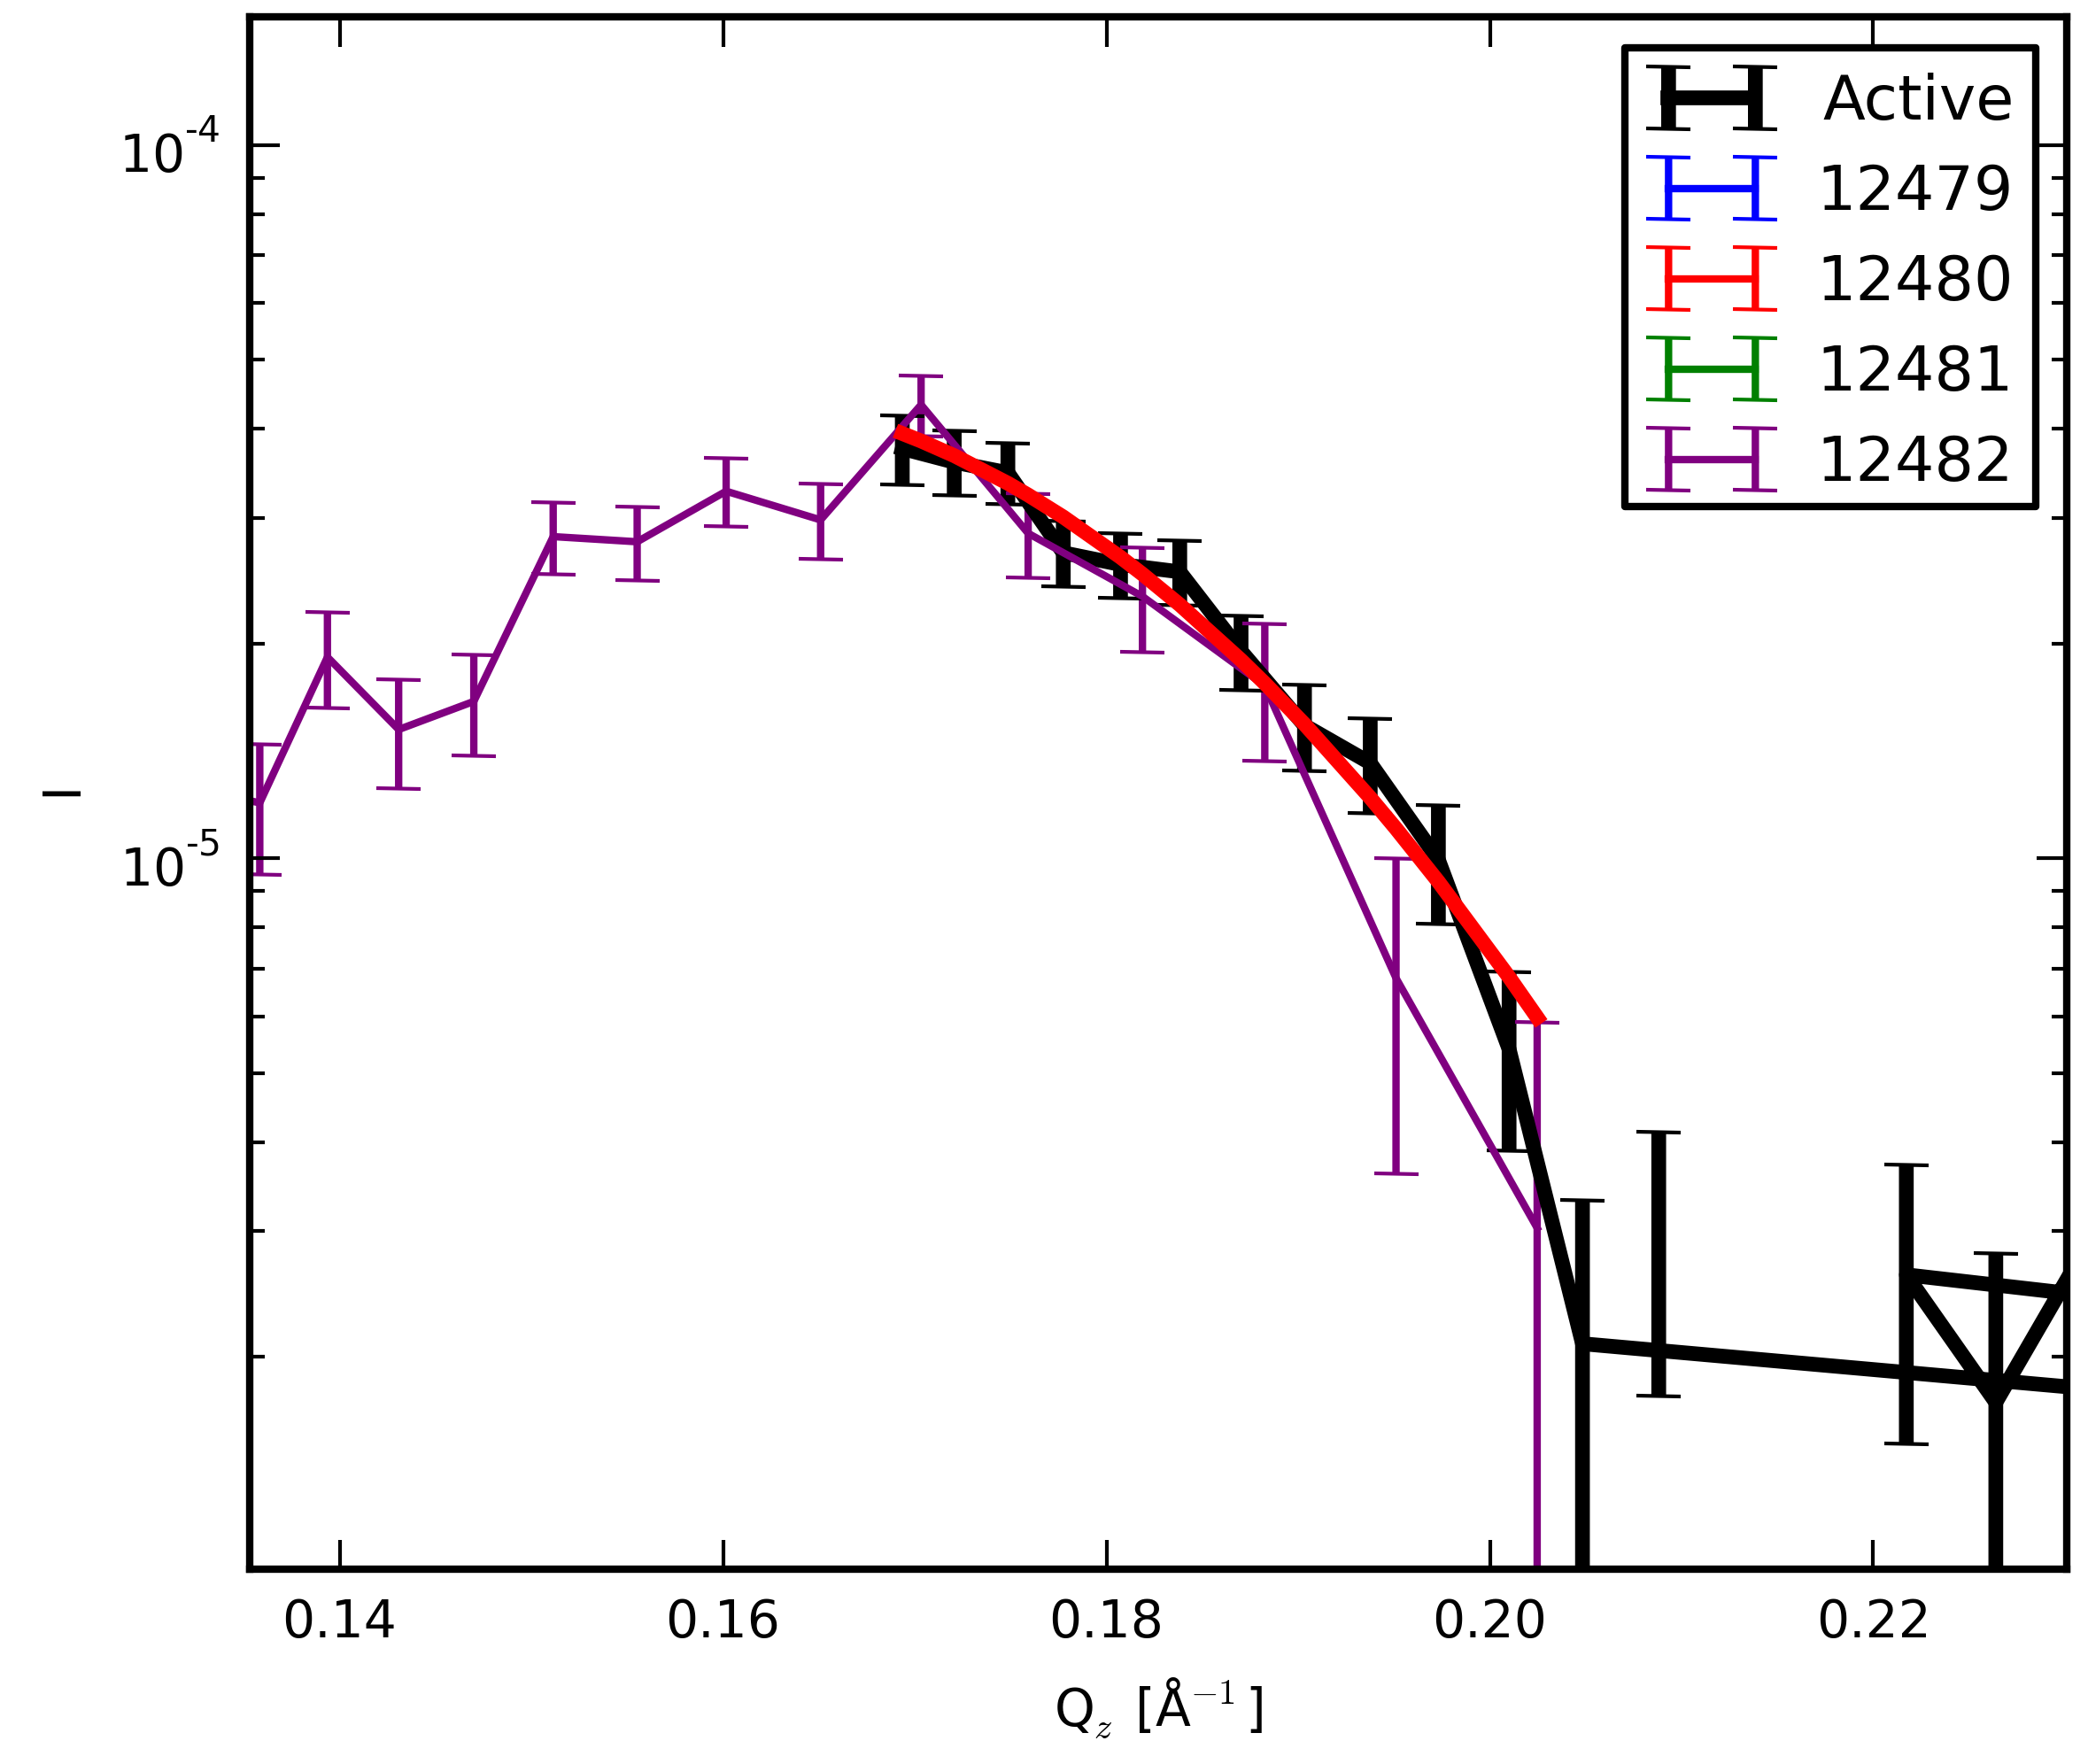
\includegraphics[width=175pt]{screenshots/stitching1.png} 
    \end{wrapfigure}
    Now you can continue adding each subsequent dataset one after another.
    If nothing goes wrong, the only thing that needs to be changed from dataset are the \textbf{Cut Pts} and \textbf{Scaling} values.
    If the scaling of subsequent datasets does not fit, activate the \textbf{Set Scaling action} \icon{totalReflection} again. 
    This fits a polynomial to the logarithmic data of both adjacent datasets including a scaling factor for the second, which is than used for the scaling after the fit.
    The error weighted $\chi^2$ used for this refinement is:
    \begin{eqnarray*}
      \chi_{stitch}^2 =& \underset{DS1}{\sum} \frac{(\log(I_i)-p(Q_i))^2}{(\delta{}I_i/I_i)^2} + \underset{DS2}{\sum} \frac{(\log(I_j\cdot scale)-p(Q_j))^2}{(\delta{}I_j/I_j)^2} \\
      \text{with } p(Q) =& a\cdot Q^2 + b\cdot Q +c \text{ for polynom order 3}
    \end{eqnarray*}
    The resulting fit function is shown in the reflectivity plot together with the scaled data as can be seen in the figure on the right.
    For some datasets with very sharp features like multilayer Bragg-peaks this method will not work, in those cases you need to change the \textbf{Scale 10\^} parameter manually until the datasets fit together nicely.
    For polarized measurements it can sometimes be helpful to switch back and forth between different polarization channels as the variation in contrast can lead to smooth transitions, where the other channel has a sharp feature.
    Now add the dataset to the reduction list with \textbf{Keep Item in List action} \icon{addRef} again and repeat the procedure for all datasets belonging to this measurement.


  \subsection{Step 5: Refine the reflectivity scaling and cutting}
  \label{sec:scaling}
    \begin{wrapfigure}[10]{r}{0.6\textwidth}
    \centering
    \begin{tabular}{cc}
       As added to reduction list& With changed cut points\\
     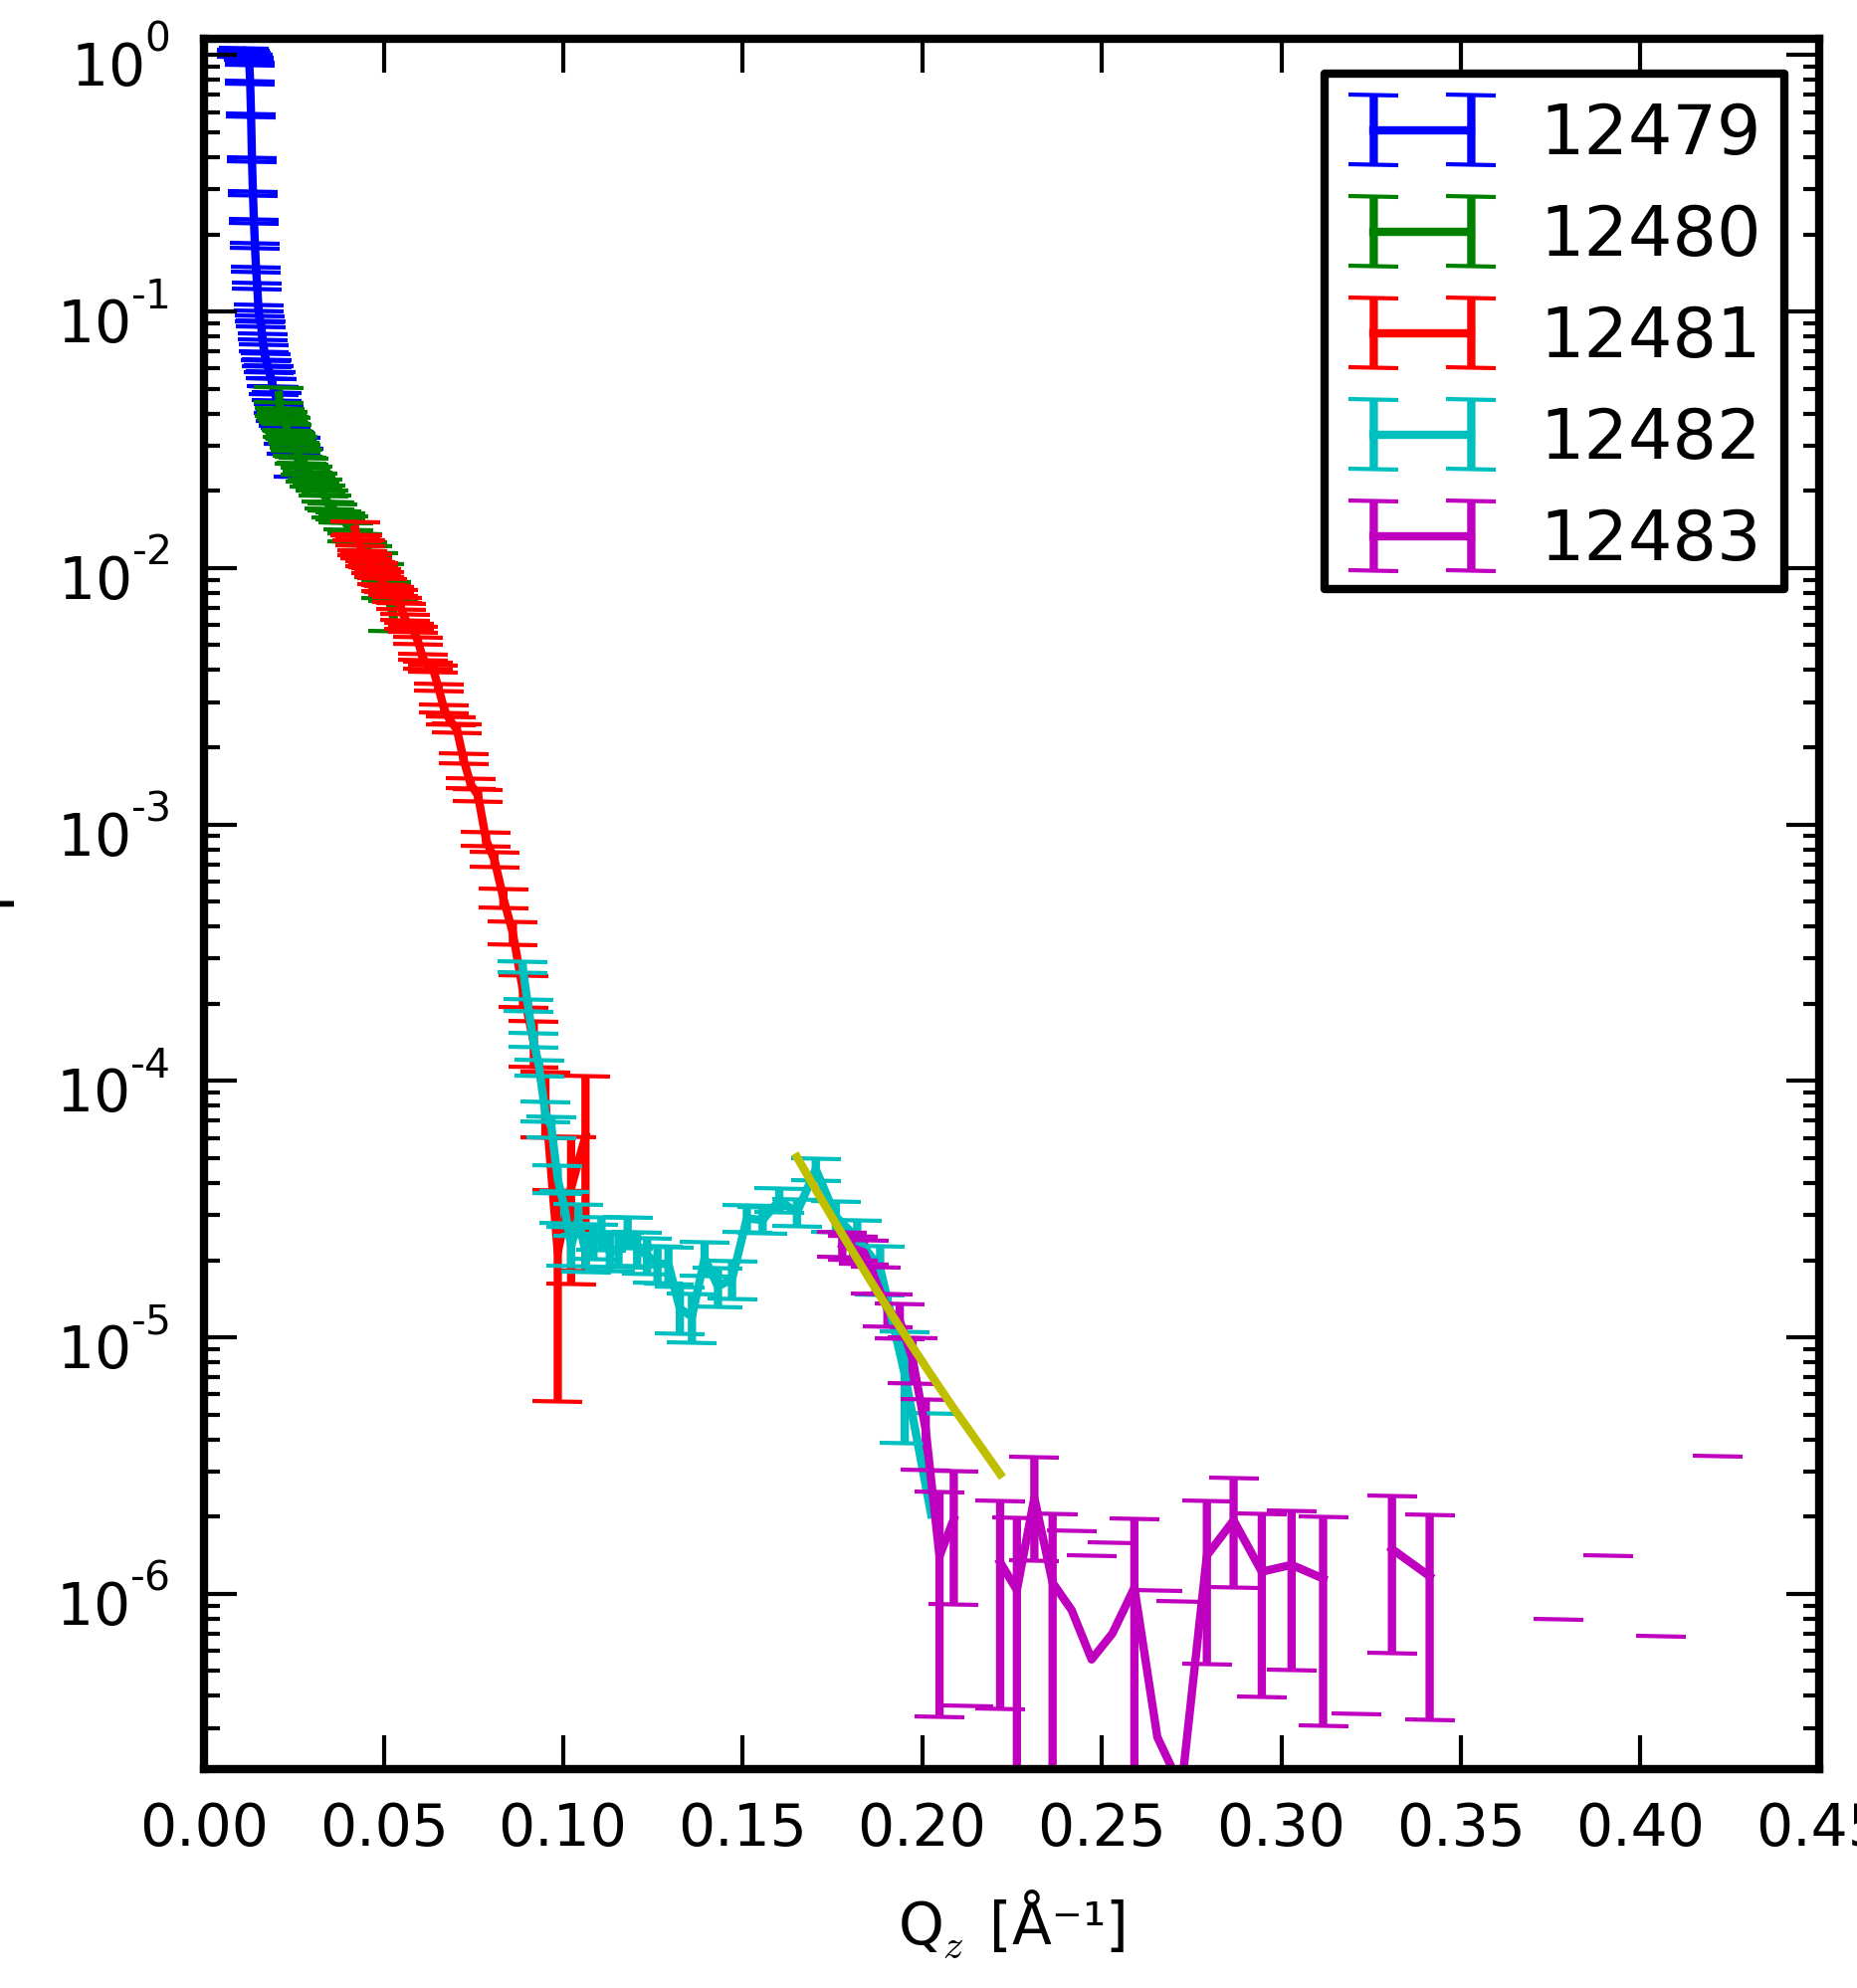
\includegraphics[width=129pt]{screenshots/stitching2.png} &
     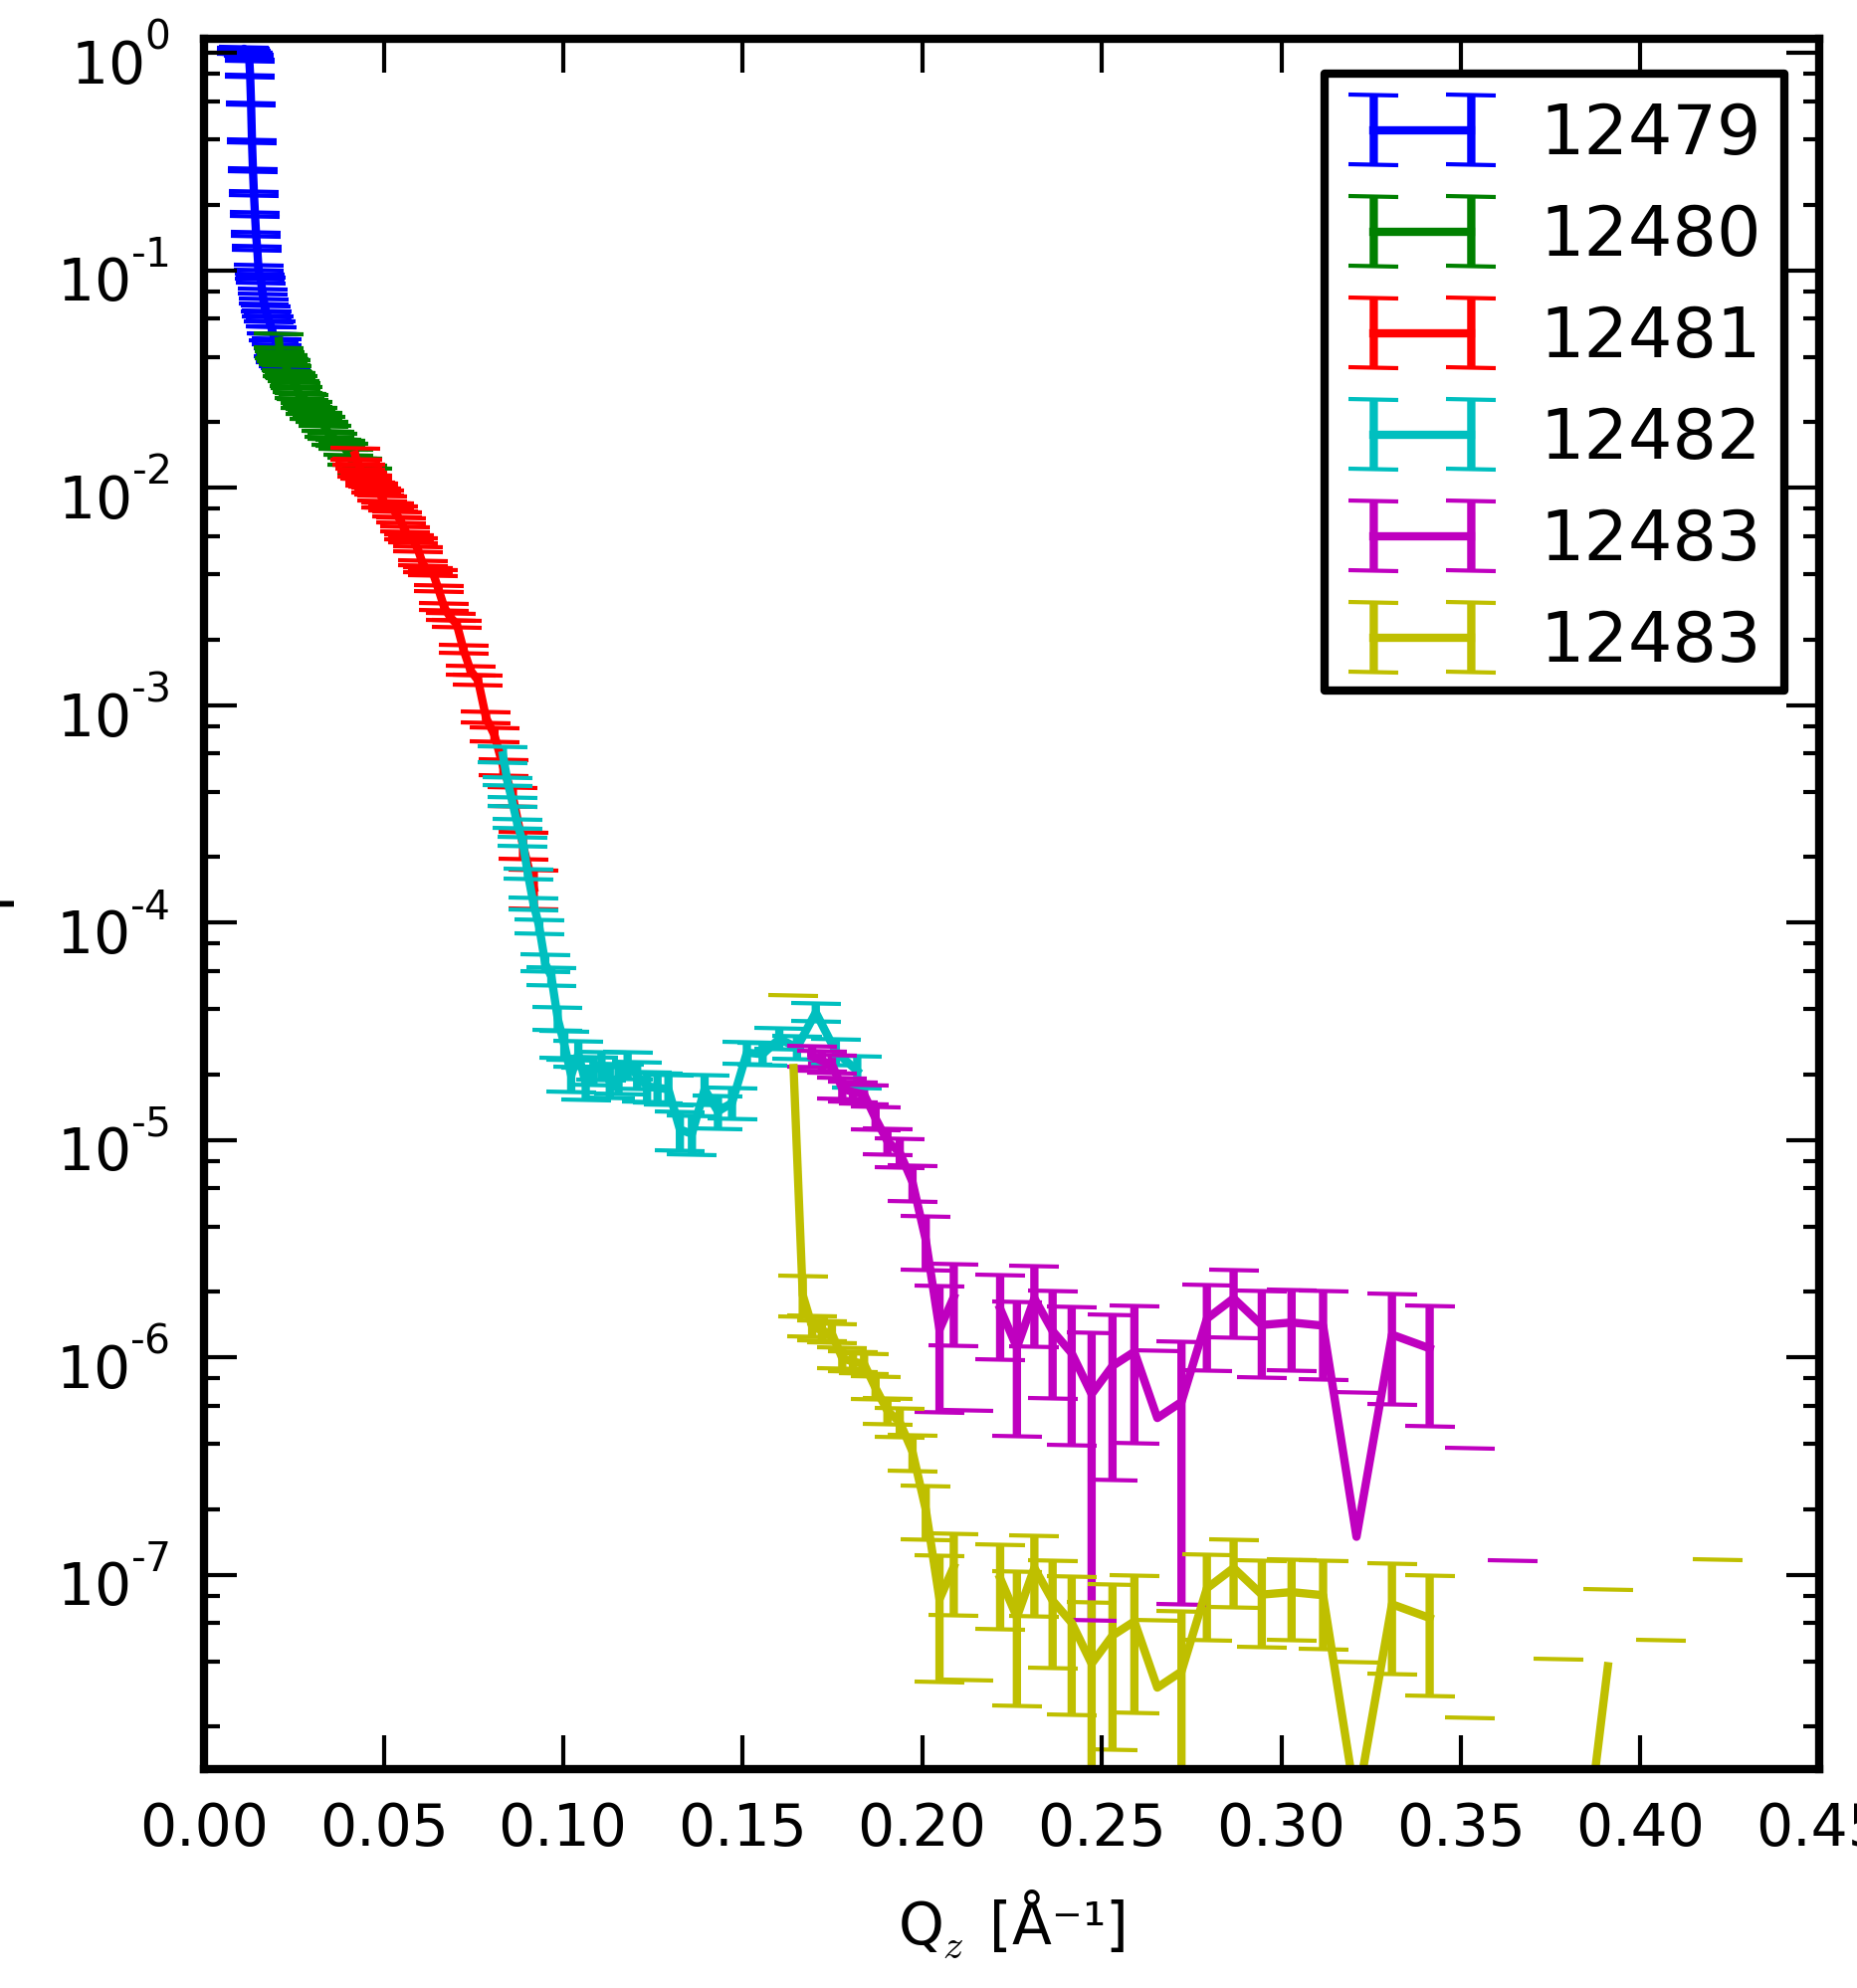
\includegraphics[width=129pt]{screenshots/cleanpoints.png} 
    \end{tabular}
    \end{wrapfigure}
    When all datasets of one measurement have been added, as can be seen in the image on the right, you can try to improve the scaling of the different parts, if needed, and change the cutting parameters.
    To change the scaling of one dataset you can either change the value of the \textbf{I0 column} entry in the reduction list or move the mouse \textbf{cursor on top of the curve} you want to scale and \textbf{move the mouse wheel}.
    To remove unwanted point you need to change the values of the \textbf{NL} and \textbf{NR column} entries as they define the number of points cut from the low- and hight-Q side respectively.
    If the number of time of flight channels in the histogram dataset is larger than the wavelength window used for the measurement it is possible that large values are needed (<=60) to see changes in the dataset.
    
\subsection{Step 6: Export your data}
  \label{sec:export}
    \begin{wrapfigure}[14]{r}{0.35\textwidth}
    \centering
     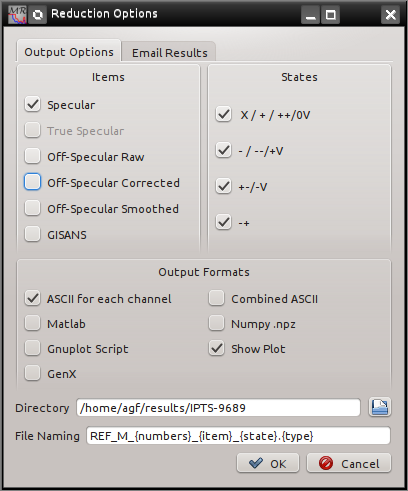
\includegraphics[width=150pt]{screenshots/reduced.png}
    \end{wrapfigure}
    Now you are ready to export you reflectivity! 
    Activate the \textbf{Reduce... action} \icon{reduce} from the menu, toolbar or the button below the reduction list.
    The reduce dialog has several options for the export of the dataset.
    You can select which reductions should be stored, choose the channels to export and define which data formats should be created.
    As a default, the specular reflectivity of all available channels will be exported to separate ASCII files and a dialog with a plot of the resulting data will be shown afterwards.
    Additional output options are a combined ASCII file containing all channels, a matlab or numpy datafile for later processing, a Gnuplot script and image file to plot the ASCII data and a GenX reflectivity modeling template already containing the measured data.
    If you want to send the resulting data to your email address you can use the \textbf{Email Results} tab to enter your address and select which and if the data should be send after the export.
    
    

\section{Examples}
  This section will give three example datasets, which you can use to try the reduction yourself and compare the result with the images in this manual.
  
\section{Common problems to be aware of}
